\documentclass[11pt]{article}

% Page geometry & typography
\usepackage[a4paper,margin=1in]{geometry}
\usepackage{lmodern}
\usepackage[T1]{fontenc}
\usepackage[utf8]{inputenc}
\usepackage{microtype}          % better kerning/justification

% Math & symbols
\usepackage{amsmath,amssymb,amsfonts}
\usepackage{amsthm}
\usepackage{mathtools} % gives \coloneqq, \DeclarePairedDelimiter, etc.
\usepackage{bm}
\usepackage{siunitx}            % \SI{...}{MW}, etc.
\sisetup{detect-all}

% Colors, hyperlinks
\usepackage{xcolor}
\definecolor{linkblue}{RGB}{0,85,160}

\usepackage{hyperref}
\hypersetup{
  colorlinks=true,
  linkcolor=linkblue,
  citecolor=linkblue,
  urlcolor=linkblue
}
\pdfstringdefDisableCommands{%
  \def\ASCDE{ASCDE}%
  \def\UEVF{UEVF}%
  \def\VOLL{VOLL}%
  \def\LOLE{LOLE}%
  \def\EUE{EUE}%
  \def\ELCC{ELCC}%
  \def\MRV{MRV}%
  \def\UCAP{UCAP}%
  \def\PRM{PRM}%
  \def\RV{RV}%
  \def\boldsymbol#1{#1}%
}

% Lists, tables, captions
\usepackage{enumitem}           % compact, customizable lists
\setlist[itemize]{leftmargin=1.25em}
\setlist[enumerate]{leftmargin=1.5em}
\usepackage{booktabs}           % professional tables
\usepackage{tabularx}           % auto-width columns
\usepackage{threeparttable}     % notes under tables
\usepackage{multirow}
\usepackage{makecell}           % line breaks in table cells
\usepackage{array}
\usepackage{caption}
\usepackage{subcaption}         % subfigures
\usepackage{float}              % [H] float placement
\usepackage{graphicx}           % figures
\usepackage{wrapfig}

% Graphics & TikZ for flow diagrams
\usepackage{tikz}
\usetikzlibrary{
  arrows.meta,
  positioning,
  calc,
  shadows.blur,
  shapes.geometric
}

% For checkmarks/crosses in comparison tables
\usepackage{pifont}
\newcommand{\cmark}{\textcolor{teal!60!black}{\ding{51}}}
\newcommand{\xmark}{\textcolor{red!70!black}{\ding{55}}}

\theoremstyle{plain}         % italic body, bold head
\newtheorem{proposition}{Proposition}[section]
\newtheorem{lemma}{Lemma}[section]
\newtheorem{theorem}{Theorem}[section]

\theoremstyle{definition}    % upright body
\newtheorem{definition}{Definition}[section]
% Better URL breaking
\usepackage{xurl}

% Bibliography (if you use biblatex; otherwise swap for natbib)
\usepackage[backend=biber,style=authoryear,maxcitenames=2,maxbibnames=10,doi=false,isbn=false,url=true]{biblatex}
% \addbibresource{refs.bib}

% Convenience macros (expand as needed)
\DeclareRobustCommand{\ASCDE}{\textsc{ascde}}
\DeclareRobustCommand{\UEVF}{\textsc{uevf}}
\DeclareRobustCommand{\VOLL}{\textsc{voll}}
\DeclareRobustCommand{\LOLE}{\textsc{lole}}
\DeclareRobustCommand{\EUE}{\textsc{eue}}
\DeclareRobustCommand{\ELCC}{\textsc{elcc}}
\DeclareRobustCommand{\MRV}{\textsc{mrv}}
\DeclareRobustCommand{\UCAP}{\textsc{ucap}}
\DeclareRobustCommand{\PRM}{\textsc{prm}}
\DeclareRobustCommand{\RV}{\textsc{rv}}
\DeclareRobustCommand{\MC}{\mathrm{MC}}

% Convenience: highlighted boxes (for callouts/policy boxes)
\usepackage[most]{tcolorbox}
\tcbset{
  enhanced,
  boxrule=0.5pt,
  colback=gray!5,
  colframe=black!25,
  arc=2pt,
  left=6pt,right=6pt,top=6pt,bottom=6pt
}

% Captions formatting
\captionsetup{font=small,labelfont=bf}

\begin{document}

\begin{center}
  {\LARGE \textbf{Incentivizing AI-Optimized Networking for Grid-Aligned Data Centers:}}\\[4pt]
  {\Large \textbf{A \UEVF/\ASCDE Policy Framework for ISOs}}\\[8pt]
  {\normalsize August 2025}
\end{center}

\vspace{0.5em}
\noindent\textbf{Authors:} Justin Candler; Uriel

\vspace{1.0em}
\begin{abstract}
\noindent
This white paper develops a structured ISO/RTO incentive framework tailored to the emergence of hyperscale, AI-driven data centers whose electrical and networking characteristics (e.g., NVIDIA Spectrum-X fabrics) present both new risks and new flexibilities for bulk power systems. Building on NERC’s 2025 Reliability Issues Steering Committee (RISC) priorities, we embed these engineered digital loads into a unified adequacy valuation ledger---the Unified Energy Valuation Framework (\UEVF) and the Adjusted System Cost of Delivered Electricity (\ASCDE). The framework expresses probabilistic reliability (\LOLE, \EUE) in monetized terms via \VOLL, enabling direct comparison of load flexibility, transmission investment, and generation adequacy within a single \$/MWh metric. 

We propose incentive mechanisms across the interconnection, capacity accreditation, demand response, and transmission pricing stack, consistent with recent MISO Business Practice Manuals on Demand Response (BPM-026) and Transmission Pricing (BPM-021). The design introduces: (i) portfolio-based deliverability rights at points of interconnection, (ii) seasonal accreditation credits for forecastable and interruptible large loads, (iii) queue triage via marginal reliability value (MRV/eMRV), and (iv) scarcity pricing aligned with operating reserve demand curves indexed to expected unserved energy. Transmission and interregional policy extensions treat transfer capability as a reliability asset, priced through $\Delta \EUE \times \VOLL$ in parity with generation and flexible load. 

The result is a coherent ISO/RTO policy blueprint that aligns hyperscale AI demand with grid adequacy, minimizes expected outage costs, and creates transparent scorecards for regulators (FERC, OMS, NARUC) and stakeholders. By embedding engineered digital loads into monetized adequacy metrics, this work establishes the foundation for reliability-consistent siting, interconnection, and market participation of next-generation AI infrastructure.
\end{abstract}

\newpage

\tableofcontents
\newpage

%=============================
\section{Executive Summary}

Artificial intelligence--driven data centers are emerging as \textbf{first-order reliability drivers} for North American bulk power systems. Their \textbf{lumpy, indivisible, and geographically concentrated load profiles} introduce adequacy and deliverability stresses that existing probabilistic planning metrics (LOLE, PRM) fail to capture. In short-run dispatch, a 600-MW hyperscale data center is ``just another load.'' In long-run adequacy and transmission planning, however, such an increment can flip an entire substation bank, trigger multi-hundred-million-dollar transmission reinforcements, or shift the regional peak by itself. 

\subsection*{The Gap in Legacy Adequacy Reporting}
\begin{itemize}
    \item \textbf{Planning Reserve Margin (PRM)} and \textbf{Loss of Load Expectation (LOLE)} are the canonical adequacy benchmarks. Yet both were designed for thermal-dominated, diversified load systems.
    \item LOLE counts the \emph{frequency} of shortage events but not their \emph{severity}. A single 1-hour curtailment and a multi-day weather-driven deficit contribute equally to the LOLE ledger~\cite{uevf_exec938}.
    \item PRM provides a static percentage buffer (e.g., 15\%) but does not link incremental adequacy risk to its economic consequences. It obscures whether additional MW are worth their cost at the margin~\cite{miso_bpm941}.
    \item Current RA manuals confirm this limitation: MISO uses LOLE for PRM calibration, with EUE visible only in transmission studies, and VOLL absent altogether from adequacy clearing~\cite{miso_bpm941}.
\end{itemize}

\subsection*{The Corrective Solution}
The \textbf{Unified Energy Valuation Framework (UEVF)} and the \textbf{Adaptive System Capacity and Deliverability Evaluation (ASCDE)} provide a harmonized valuation language:
\begin{itemize}
    \item \textbf{EUE (Expected Unserved Energy)} captures adequacy severity.
    \item \textbf{VOLL (Value of Lost Load)} monetizes that severity into \$/MWh avoided outage cost.
    \item \textbf{$\EUE \times \VOLL = \text{Reliability Value}$} becomes an explicit annualized \$/year ledger of outage risk, directly comparable to capacity and transmission costs~\cite{uevf_exec938}.
    \item \textbf{ASCDE} integrates this monetized reliability layer with dispatch, storage, transmission, and market value---yielding a system-level \$/MWh ``all-in'' cost of delivered electricity~\cite{uevf_cross942}.
\end{itemize}

Embedding EUE $\times$ VOLL into PRM setting, transmission scoring, and interconnection triage allows ISOs to:
\begin{enumerate}
    \item Translate adequacy risk into a transparent monetary value.
    \item Rank resources and projects by avoided outage cost per MW.
    \item Provide policymakers and regulators with a unified cost--risk trade-off tool, replacing heuristic buffers with economically grounded adequacy decisions.
\end{enumerate}

\subsection*{Policy-Maker Summary Table: Today vs. UEVF/ASCDE}
\begin{table}[H]
\centering
\caption*{Comparison of Legacy Adequacy Metrics and UEVF/ASCDE Approach}
\begin{tabular}{|p{4cm}|p{5.5cm}|p{6cm}|}
\hline
\textbf{Dimension} & \textbf{Today: PRM / LOLE} & \textbf{UEVF / ASCDE} \\
\hline
Adequacy Standard & LOLE $\leq$ 0.1 days/yr; PRM = \% above peak & LOLE + EUE integrated, monetized into \$/yr via VOLL~\cite{uevf_exec938} \\
\hline
Risk Measured & Frequency only (event count) & Frequency + severity (MWh unserved) + economic impact (\$/MWh)~\cite{uevf_cross942} \\
\hline
Economic Linkage & Implicit; no direct cost tie & Direct: Reliability Value = EUE $\times$ VOLL (\$/yr) \\
\hline
Project Valuation & MW crediting only (UCAP/ELCC) & Marginal reliability value (\$/MW-yr) informs queue triage and PRM calibration~\cite{uevf_exec938} \\
\hline
Comparability Across ISOs & Fragmented: PJM (IRM), CAISO (ELCC), ERCOT (energy-only) & Harmonized: Standardized VOLL; single ASCDE metric across ISOs~\cite{uevf_cross942} \\
\hline
\end{tabular}
\end{table}

\bigskip
This reorientation moves adequacy from heuristic reserve margins toward a transparent, monetized risk framework. It equips policymakers with a tool to judge whether the next MW of capacity, transmission, or demand flexibility is worth its cost in terms of avoided outage risk.
\subsection*{What Changes for Policymakers}
\begin{itemize}
  \item \textbf{Publish monetized adequacy alongside LOLE/PRM.} Require seasonal, locational \EUE\ bands and a standardized \VOLL{} (e.g., $10$--$25$ k$/\,\mathrm{MWh}$) to disclose \emph{expected outage cost (\$/yr)} by LRZ/zone.
  \item \textbf{Rank projects and portfolios by avoided outage cost.} Use \emph{marginal reliability value} $\MRV = -\partial\EUE/\partial\text{Cap} \times \VOLL$ (\$/MW-yr) and its deliverability-adjusted form (eMRV = $\MRV\,\cdot D_\ell$) to triage queues, target transmission, and set \PRM{} economically.
  \item \textbf{Create a Large-Load RA class.} Treat engineered data center loads $>\!200\,\mathrm{MW}$ as a market class with telemetry, forecastability SLAs, interruptible blocks, and seasonal credits tied to \EUE\ reduction.
  \item \textbf{Adopt \ASCDE{} in IRPs/RA filings.} Report the \emph{system} $\$/\mathrm{MWh}$ cost that includes dispatch, storage, transmission, \emph{and} monetized reliability (\EUE$\times$\VOLL), so resource rankings reflect \emph{delivered} value.
\end{itemize}

\subsection*{12-Month Action Plan}
\begin{enumerate}
  \item \textbf{Disclosure rule:} add seasonal/locational \EUE\ and \VOLL\ bands to RA/IRP filings; publish \ASCDE{} module breakdowns per portfolio.
  \item \textbf{Pilot:} compute and publish \MRV/eMRV scorecards for interconnection/\emph{ARQ} triggers; fast-track top-decile projects.
  \item \textbf{Tariff/BPM light-touch:} define a Large-Load RA class (telemetry, forecast, interruptible hours, performance settlement) without overhauling core markets.
  \item \textbf{Transmission scoring:} include a first-class benefit term $\Delta\EUE\times\VOLL$ (native + standardized \VOLL) alongside production cost savings.
\end{enumerate}

\subsection*{KPIs and Disclosures}
\begin{itemize}
  \item Seasonal \EUE\ (MWh/yr) and \emph{Reliability Value} (\$/yr) by LRZ/zone; sensitivity at \VOLL $=\{10, 17, 20, 25\}\,$k$/\,\mathrm{MWh}$.
  \item Queue \emph{eMRV} distribution and cumulative \emph{avoided outage cost} for top-ranked projects.
  \item \ASCDE{} by resource/portfolio with module deltas (dispatch, storage, transmission, reliability, market value).
\end{itemize}

\subsection*{Illustrative Flow (Measurement Pipeline)}

\begin{figure}[H]
  \centering
  % auto-shrink to textwidth to avoid overflow on any page size
  \resizebox{\textwidth}{!}{%
  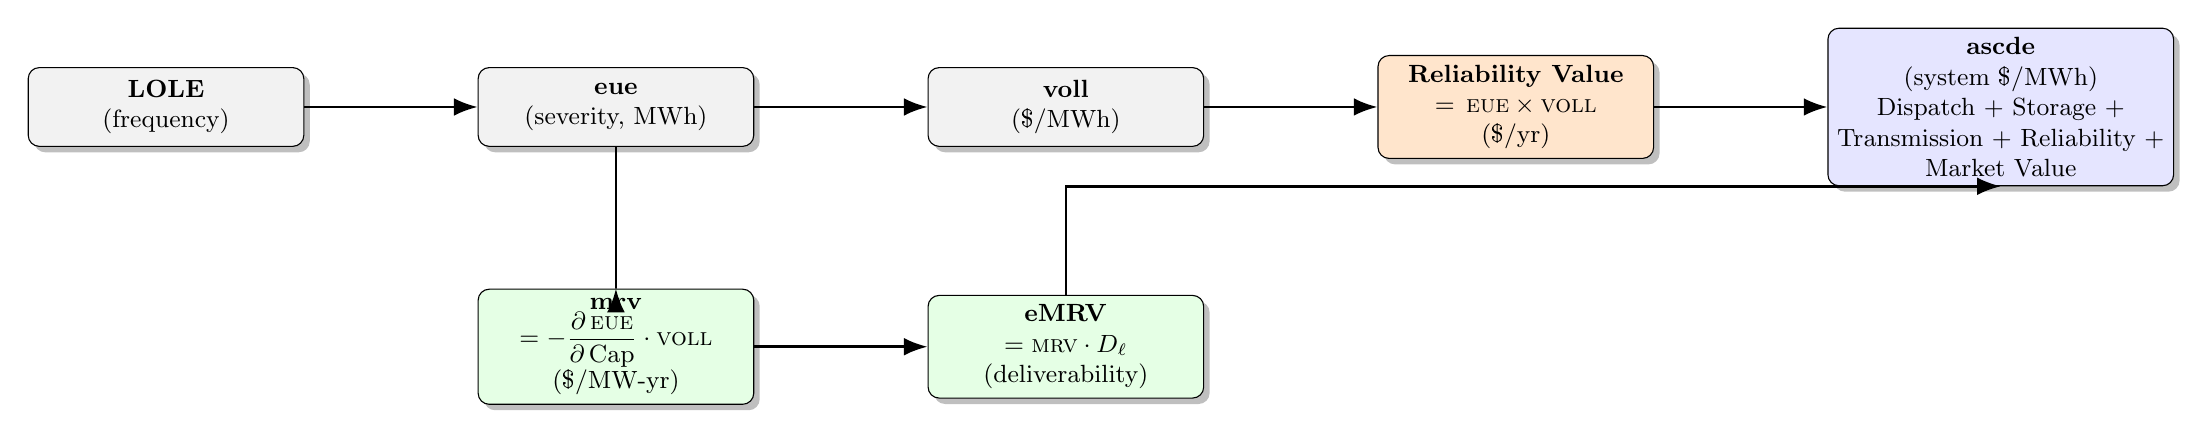
\begin{tikzpicture}[
    node distance=2.2cm,
    every node/.style={font=\small},
    box/.style={
      draw,
      rounded corners,
      align=center,
      fill=gray!10,
      minimum width=35mm,
      minimum height=10mm,
      drop shadow
    },
    ar/.style={-{Latex[length=3mm]}, line width=0.9pt}
  ]
    % top chain: LOLE -> EUE -> VOLL -> Reliability Value -> ASCDE
    \node[box] (lole) {\textbf{LOLE}\\(frequency)};
    \node[box, right=of lole] (eue) {\textbf{\EUE}\\(severity, MWh)};
    \node[box, right=of eue] (voll) {\textbf{\VOLL}\\(\$/MWh)};
    \node[box, right=of voll, fill=orange!20] (rv)
      {\textbf{Reliability Value}\\$=\,\EUE\times\VOLL$\\(\$/yr)};
    \node[box, right=of rv, fill=blue!10] (ascde)
      {\textbf{\ASCDE}\\(system \$/MWh)\\Dispatch + Storage +\\ Transmission + Reliability +\\ Market Value};

    % arrows along the top
    \draw[ar] (lole) -- (eue);
    \draw[ar] (eue) -- (voll);
    \draw[ar] (voll) -- (rv);
    \draw[ar] (rv) -- (ascde);

    % lower branch: MRV -> eMRV feeding into ASCDE
    \node[box, below=1.8cm of eue, fill=green!10] (mrv)
      {\textbf{\MRV}\\$=-\dfrac{\partial\,\EUE}{\partial\,\mathrm{Cap}}\cdot\VOLL$\\(\$/MW-yr)};
    \node[box, right=of mrv, fill=green!10] (emrv)
      {\textbf{eMRV}\\$=\MRV\cdot D_{\ell}$\\(deliverability)};

    \draw[ar] (eue.south) |- (mrv.north);
    \draw[ar] (mrv) -- (emrv);
    \draw[ar] (emrv.north) |- (ascde.south);

  \end{tikzpicture}%
  }
  \caption{From probabilistic adequacy to monetized risk and unified valuation. The lower branch supplies project/portfolio ranking for queue triage (\MRV, eMRV).}
\end{figure}

\subsection*{Caveats and Guardrails}
\begin{itemize}
  \item \textbf{Avoid double counting.} If deliverability derates are applied in \ELCC/\UCAP{}, do not re-apply full upgrade costs as a separate surcharge in \ASCDE.
  \item \textbf{Report bands, not points.} Publish \VOLL{} bands and stochastic ranges for \EUE{} to avoid spurious precision.
  \item \textbf{Seasonal first.} Annual averages can mask spring/winter adequacy shocks; always report seasonal \ASCDE{} and \EUE{}.
\end{itemize}

\section*{2. Introduction \\ \large Context, Risk Taxonomy, and Measurement Gaps}

\subsection*{2.1 NERC 2025 Risk Taxonomy: What Changed and Why It Matters}
The North American reliability posture is being reshaped by four interacting drivers that together invalidate historic planning heuristics:
\begin{enumerate}[label=\textbf{(R\arabic*)}, leftmargin=2.25em]
  \item \textbf{Grid transformation.} Rapid substitution of synchronous thermal units with inverter-based resources (IBR), growth in limited-duration storage, and steep load additions from \emph{engineered} digital loads (AI data centers, hyperscalers, crypto) are altering adequacy from a \emph{capacity} sufficiency problem to an \emph{energy/time/location} sufficiency problem. Seasonal and hourly correlation effects dominate portfolio risk.
  \item \textbf{Resilience to extreme events.} NERC reframes resilience as an \emph{all-hazards} problem: long-duration meteorology (cold snaps, heat domes, smoke), coincident with cyber/physical events and supply-chain constraints. The salient metric shifts from deterministic \PRM{} to probabilistic tail-risk \emph{exposure and recovery time}. 
  \item \textbf{Critical infrastructure interdependencies.} Gas-electric and communications-power couplings now act as first-order constraints on generation availability and system observability. Reliability must explicitly price the risk of just-in-time gas interruption and communications outages.
  \item \textbf{Energy policy volatility.} Misaligned timelines across siting, interconnection, incentives, and retirement schedules convert policy into a reliability risk amplifier. Queue backlogs and permitting delays convert “paper MW” into \emph{phantom adequacy}. 
\end{enumerate}
These drivers are not separable; they form a coupled system in which the \emph{location, timing, and recoverability} of energy deliveries dominate the adequacy function. Any framework that continues to evaluate reliability on an annualized \PRM{} basis undercounts the risk surface and misallocates capital.

\subsection*{2.2 How AI-Optimized Networking Changes Load Physics}
\paragraph{From organic to engineered load.} Traditional system planning treated demand as weather- and behavior-driven, with stochastic variability that \emph{averages out} across geography and sector mixes. AI-optimized fabrics (e.g., Spectrum-X/XGS-class Ethernet for GPU clusters) invert this logic: loads become \emph{orchestrated}, low-variance, and \emph{coincident across sites}. Key properties:
\begin{itemize}[leftmargin=1.5em]
  \item \textbf{Temporal coherence.} Model training windows (multi-hour blocks) synchronize GPU utilization across racks, campuses, and—under cross-site fabrics—across metropolitan areas. Effective coincidence factor approaches unity during training epochs.
  \item \textbf{Spatial coherence.} Latency-optimized fabrics collapse multiple buildings/campuses into a single logical cluster. From a grid perspective, this concentrates MW at a small set of substations and EHV corridors, reducing diversity benefits and increasing \emph{N-1/N-1-1} stress.
  \item \textbf{Predictable but \emph{blocky}.} The load is forecastable at sub-hour granularity, but increments are indivisible (e.g., 50–200 MW steps per expansion), producing \emph{lumpy} network upgrades and step changes in deliverability constraints.
\end{itemize}
These characteristics transform the adequacy question from “\emph{How much MW in aggregate?}” to “\emph{Where, when, and under which contingencies can MW be delivered?}”

\subsection*{2.3 Limits of Legacy Adequacy Reporting}
\paragraph{Binary thresholds mask economic risk.} The canonical 0.1-days/year \LOLE{} standard and annual \PRM{} reporting provide a pass/fail view of reliability. They do not quantify \emph{severity} (\EUE{}) or \emph{economic impact} (\EUE\,$\times$\,\VOLL). Two systems that both meet 0.1 \LOLE{} can carry \emph{orders of magnitude} different expected outage cost.
\paragraph{Annual averages hide seasonal and locational shocks.} Seasonal \ELCC{} collapses (e.g., spring wind correlation change) can triple the required \PRM{} versus summer, even with unchanged annual \LOLE. Locational deliverability constraints convert accredited capacity (\UCAP) into “paper MW.”
\paragraph{No mechanism to price interdependencies.} Gas deliverability, communications outages, and supply-chain lead times do not appear in \PRM/\LOLE tables, yet dominate availability in stress periods.
\medskip
\noindent \emph{Conclusion:} Policymakers cannot prioritize or sequence investments with legacy metrics. A monetized, seasonal, locational adequacy ledger is required.

%=============================
\section*{3. Technical Primer: AI-Optimized Ethernet for AI Data Centers}
\subsection*{3.1 Fabric Architecture and Features}
\paragraph{Switch silicon (e.g., Spectrum-4).} High-radix, cut-through Ethernet switches with on-die congestion telemetry, adaptive routing, and hardware ECN/RED marking, enabling deterministic, microburst-resilient performance for collective communication (all-reduce, all-gather). Line rates in the 800G–1.6T class per port with co-packaged optics reduce SERDES power and thermal penalties.
\paragraph{Smart NICs/DPUs (e.g., BlueField-3 SuperNIC).} Host offload for RDMA over Converged Ethernet (RoCEv2), in-network compute for transport pacing, credit management, and telemetry export. This moves congestion control from host CPUs to NIC/ASIC, stabilizing training throughput under high fan-in traffic.

\paragraph{Software stack (NCCL/MagnumIO).} 
The NVIDIA Collective Communications Library (NCCL) and MagnumIO orchestrate topology-aware collectives optimized for the specific Clos/dragonfly/radix of the fabric. 
Performance tuning depends on \emph{end-to-end} alignment (GPU $\leftrightarrow$ NIC/PCIe $\leftrightarrow$ switch ASIC), which is why the stack behaves as a single engineered system.

\subsection*{3.2 Operational Consequences for Grid Planners}
\begin{enumerate}[label=\textbf{(C\arabic*)}, leftmargin=2.25em]
  \item \textbf{Synchronization across campuses.} With cross-site fabrics, multiple buildings behave as a \emph{single} logical cluster. Coincidence factor approaches unity during training epochs, elevating the seasonal and hourly \EUE{} in the binding LRZ/substation.
  \item \textbf{Step-changes in network loading.} Cluster scale-ups arrive in 50–200 MW quanta. Under \emph{N-1/N-1-1} screening, transformer banks and 138/230/345 kV corridors hit thermal/voltage limits abruptly, inducing high-variance upgrade costs (often six–nine figures) and \emph{deliverability derates} on accredited capacity.
  \item \textbf{Predictable profiles enable contractual flexibility.} The same orchestration that drives coincidence also enables day-ahead block commitment, interruptible hours, and telemetry SLAs—if properly incentivized. This is the lever for translating engineered load \emph{predictability} into reliability value.
\end{enumerate}

\subsection*{3.3 Siting and Energy Implications}
\paragraph{High power density and cooling.} AI racks exceed traditional power densities, driving onsite substation and thermal plant upgrades, water-use considerations, and backup generation interconnection. Thermal plumes and water availability introduce non-trivial siting externalities.
\paragraph{Clustering and geography.} Latency and supply-chain economics concentrate campuses near major metros and fiber backbones, frequently overlapping with transmission constraints. From an adequacy standpoint, cluster placement should be evaluated on an eMRV basis: sites that deliver higher \(-\partial \EUE/\partial \text{Cap})\times \VOLL\) per MW should be prioritized.
\paragraph{Portfolio design.} Cross-campus fabrics support diversified siting only if end-to-end application latencies permit. Where latency budgets are tight, campuses will co-locate, increasing the \emph{local} adequacy premium and the value of flexible load participation (interruptibility slices, ramp agreements).

\medskip
\noindent \textbf{Implication for policy design.} AI-optimized Ethernet fabrics make data center demand \emph{dispatch-like}: synchronized, schedulable, measurable. ISO incentive design should convert these properties into monetized adequacy reductions (\EUE\,$\times$\,\VOLL), \emph{not} treat them as generic firm load.


%=============================
\section*{4. UEVF: From Probabilistic Risk to Monetized Adequacy}

\subsection{From \LOLE~to \EUE~to \VOLL}

Legacy adequacy metrics such as \LOLE{} (days/yr) are frequency measures: they indicate how often capacity shortfalls are expected but say nothing about their depth or cost. For example, a single one-hour shortage in spring counts the same as a three-day polar vortex deficit. The \UEVF{} framework extends this by embedding severity and value:

\begin{equation}
\EUE = \mathbb{E}\!\left[\sum_{t} (L_t - C_t)^+ \Delta t\right] \quad [\text{MWh/yr}],
\end{equation}

where $(L_t - C_t)^+$ is unmet load. Multiplying by \VOLL{} (in \$/MWh) monetizes the adequacy gap:

\begin{equation}
\text{Reliability Value (RV)} = \EUE \times \VOLL \quad [\$/\text{yr}],
\end{equation}

which is directly comparable to capacity and transmission investment costs.

\paragraph{Historical context.} The “1 day in 10 years” standard emerged in the 1960s–1980s under thermal-dominated fleets, when a 15\% PRM roughly guaranteed LOLE $\leq 0.1$/yr. Today’s diversified, weather-driven systems demand richer risk metrics. Other regions are already evolving: ENTSO-E applies probabilistic risk ranges, Australia reports seasonal \EUE, and New Zealand integrates \VOLL{} in adequacy settings.

\paragraph{Risk distributions.} Equal annual \EUE{} values can conceal very different risk shapes. Consider two systems: one with many small events, another with rare multi-day deficits. To expose this, \UEVF{} recommends reporting \emph{Conditional Value at Risk} (CVaR):

\begin{equation}
\text{CVaR}_{\alpha} = \mathbb{E}\,[\,\EUE \mid \EUE > q_{\alpha}\,],
\end{equation}

where $q_{\alpha}$ is the $\alpha$-quantile of \EUE. This ensures tail events are visible to policymakers.

\paragraph{Cross-sector benchmarking.} A monetized \EUE$\times$\VOLL ledger aligns adequacy with practices in other network industries: insurance premiums in finance, reliability standards for gas pipelines, or telecom outage penalties. Policymakers can thus view adequacy not as an engineering artifact but as an \emph{insurance premium} against outage risk.

\subsection{\ASCDE~Master Metric}

The Adjusted System-Level Cost of Delivered Electricity (\ASCDE) is the “all-in” valuation denominator of the \UEVF:

\begin{equation}
\ASCDE = \frac{ \text{PV[Dispatch + Fuel + Storage + Transmission + Reliability + Market Value]} }{\text{Reliable MWh Delivered}}.
\end{equation}

Unlike LCOE, which ignores reliability and deliverability, \ASCDE{} integrates:

\begin{itemize}
  \item \textbf{Dispatch \& Fuel}: operating costs under SCUC/SCED.
  \item \textbf{Storage}: tail-risk trimming via \EUE{} reduction.
  \item \textbf{Transmission}: congestion relief and deliverability factors $D_\ell$.
  \item \textbf{Reliability}: monetized adequacy via \EUE{}\,$\times$\,\VOLL.
  \item \textbf{Market Value}: locational marginal pricing, ancillary service credit.
\end{itemize}

\subsection{Seasonal and Locational Extensions}

Static PRM targets obscure the time- and location-dependence of adequacy. \UEVF{} introduces:

\begin{enumerate}
  \item \textbf{Seasonal PRM}: e.g., higher winter PRM to capture heating electrification risk.
  \item \textbf{Marginal \ELCC}: dynamic accreditation by season, reflecting solar winter drop-off or wind summer lull.
  \item \textbf{Deliverability Factor $D_\ell$}: locational derating tied to nodal transmission headroom.
  \item \textbf{Tail-Risk Weighting}: explicit valuation of 95th–99th percentile \EUE{} events, aligning with insurance-style pricing.
\end{enumerate}

\begin{tcolorbox}
\textbf{Policy hook:} Moving from LOLE-only to EUE$\times$VOLL is akin to replacing a “check engine light” with a \$/yr invoice of risk. It makes trade-offs visible, actionable, and comparable across portfolios.
\end{tcolorbox}


\section*{5. Quantifying Large Load Impact in \UEVF}

\subsection{Accreditation $\times$ Deliverability $\Rightarrow$ Usable Headroom}

For large indivisible loads (e.g., 600 MW data centers), adequacy impact is not proportional but lumpy. \UEVF{} reframes their contribution as:

\begin{equation}
\text{Usable Headroom} = \text{ELCC} \times \text{Nameplate MW} \times D_\ell,
\end{equation}

where $D_\ell$ captures substation and transmission limits. Lumpiness means incremental adequacy impacts scale non-linearly:

\[
\Delta \EUE(\Delta L) \approx 
\begin{cases}
\epsilon, & \Delta L \text{ small, dispersed} \\
\text{step increase}, & \Delta L \text{ large, indivisible.}
\end{cases}
\]

\subsection{Marginal Reliability Value (\MRV) and Effective MRV (eMRV)}

The \MRV{} formalizes the dollar value of avoided outage risk per added MW:

\begin{equation}
\MRV = -\frac{\partial \EUE}{\partial \text{Capacity}} \times \VOLL \quad [\$/MW\text{-yr}],
\end{equation}

and when deliverability is included:

\begin{equation}
\text{eMRV} = \MRV \times D_\ell.
\end{equation}

This gives planners a transparent screening metric: add capacity only if its marginal cost $<\MRV$. For large new loads, eMRV highlights when incremental adequacy cost per MW exceeds the system benefit of additional infrastructure.

\paragraph{Unit commitment effects.} Even if peak does not rise, a flat 600 MW block can shift unit commitment economics by forcing must-run gas units through low-demand hours. Additional cost can be expressed as:

\begin{equation}
\Delta \text{UC Cost} = \sum_{g} C^{\text{start}}_g \cdot \Delta \text{starts}_g.
\end{equation}

\subsection{Value of Forecastability and Load Shaping}

AI-optimized data centers exhibit relatively flat baseload demand, but \UEVF{} emphasizes that their system impact depends on forecastability and controllability:

\begin{itemize}
  \item \textbf{Telemetry APIs}: sub-hour visibility lowers uncertainty, reducing reserve needs.
  \item \textbf{Sub-hour Profiles}: shaping load (e.g., batch scheduling or AI job deferral) flattens peaks, cutting \EUE.
  \item \textbf{Interruptibility Slices (ICC)}: if $x$\% of load is contractually curtailable, it is valued as negative \EUE. 
  \item \textbf{Shaping Value (SV)}: reduction in ramp rate (MW/min) relative to baseline, valued via avoided reserve cost.
\end{itemize}

\paragraph{Reliability vs. efficiency trade-off.} Large loads can reduce balancing reserve needs (smoother profile) but increase adequacy and transmission costs (lumpy increments). A two-axis framework captures this: one axis for volatility reduction, one for headroom pressure.

\begin{tcolorbox}
\textbf{Policy hook:} A 600 MW hyperscale facility is not automatically a liability. If 20\% is interruptible and telemetry-certified, \UEVF{} shows its reliability value could rival a mid-sized peaker.
\end{tcolorbox}

% Large‑Load Valuation Flow (ELCC → MRV → eMRV → ASCDE)
% Requires in preamble:
% \usepackage{tikz}
% \usetikzlibrary{arrows.meta,positioning,shadows.blur,calc}
% Optional: \usepackage{float} for [H]

\begin{figure}[H]
  \centering
  \resizebox{\textwidth}{!}{%
  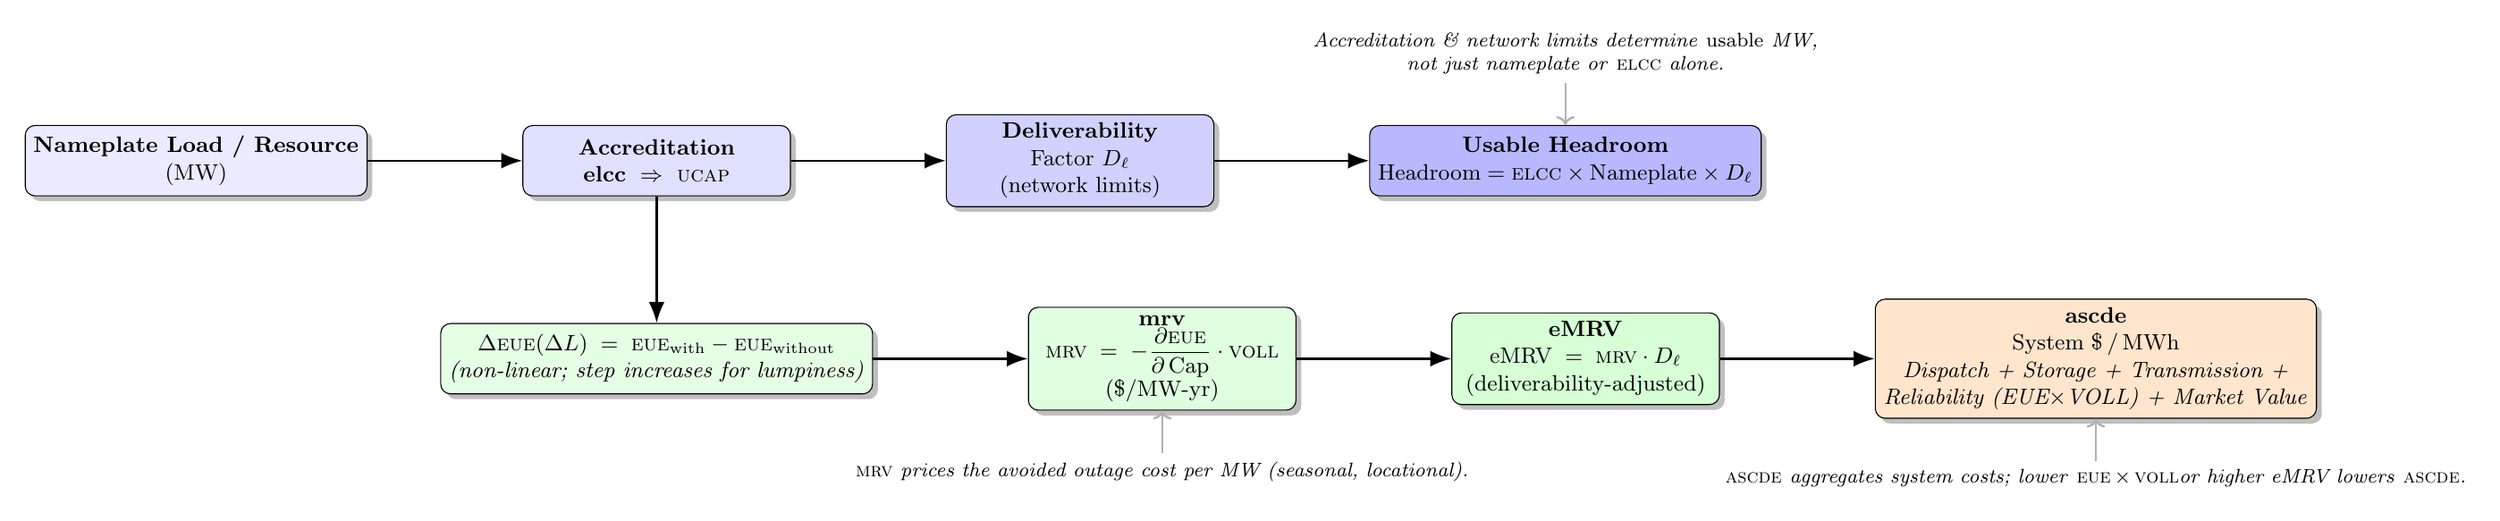
\begin{tikzpicture}[
    node distance=2.2cm,
    every node/.style={font=\small},
    box/.style={
      draw,
      rounded corners,
      align=center,
      fill=gray!10,
      minimum width=38mm,
      minimum height=10mm,
      drop shadow
    },
    note/.style={
      draw=none,
      align=center,
      font=\footnotesize\itshape
    },
    ar/.style={-{Latex[length=3mm]}, line width=0.9pt}
  ]

    % Top: Nameplate & Accreditation → Usable Headroom (w/ D_ell)
    \node[box, fill=blue!8] (name) {\textbf{Nameplate Load / Resource}\\(MW)};
    \node[box, right=of name, fill=blue!12] (elcc)
      {\textbf{Accreditation}\\\textbf{\ELCC} $\;\Rightarrow\;$ \UCAP};
    \node[box, right=of elcc, fill=blue!18] (deliver)
      {\textbf{Deliverability}\\Factor $D_{\ell}$\\(network limits)};
    \node[box, right=of deliver, fill=blue!28] (usable)
      {\textbf{Usable Headroom}\\$\text{Headroom} = \ELCC \times \text{Nameplate} \times D_{\ell}$};

    \draw[ar] (name) -- (elcc);
    \draw[ar] (elcc) -- (deliver);
    \draw[ar] (deliver) -- (usable);

    % Lower branch: ΔEUE → MRV → eMRV → ASCDE
    \node[box, below=1.8cm of elcc, fill=green!10] (deue)
      {$\displaystyle \Delta \EUE(\Delta L)\;=\;\EUE_{\text{with}}-\EUE_{\text{without}}$\\
       \textit{(non‑linear; step increases for lumpiness)}};
    \node[box, right=of deue, fill=green!12] (mrv)
      {\textbf{\MRV}\\$\displaystyle \MRV\;=\;-\frac{\partial \EUE}{\partial\,\text{Cap}}\cdot \VOLL$\\(\$/MW‑yr)};
    \node[box, right=of mrv, fill=green!16] (emrv)
      {\textbf{eMRV}\\$\displaystyle \text{eMRV}\;=\;\MRV \cdot D_{\ell}$\\(deliverability‑adjusted)};
    \node[box, right=of emrv, fill=orange!20] (ascde)
      {\textbf{\ASCDE}\\System \$\,/\,MWh\\
       \textit{Dispatch + Storage + Transmission +}\\
       \textit{Reliability (EUE$\times$VOLL) + Market Value}};

    \draw[ar] (elcc.south) |- ($(elcc.south)!0.5!(deue.north)$) -| (deue.north);
    \draw[ar] (deue) -- (mrv);
    \draw[ar] (mrv) -- (emrv);
    \draw[ar] (emrv) -- (ascde);

    % Policy/interpretive notes
    \node[note, above=0.6cm of usable] (n1)
      {Accreditation \& network limits determine \emph{usable} MW,\\
       not just nameplate or \ELCC{} alone.};
    \node[note, below=0.6cm of mrv] (n2)
      {\MRV{} prices the avoided outage cost per MW (seasonal, locational).};
    \node[note, below=0.6cm of ascde] (n3)
      {\ASCDE{} aggregates system costs; lower \EUE\,$\times$\,\VOLL or higher eMRV lowers \ASCDE{}.};

    % Optional helper arrows from notes
    \draw[ar,->,gray!60] (n1.south) -- (usable.north);
    \draw[ar,->,gray!60] (n2.north) -- (mrv.south);
    \draw[ar,->,gray!60] (n3.north) -- (ascde.south);

  \end{tikzpicture}%
  }
  \caption{Large‑load valuation flow: Accreditation and deliverability determine \emph{usable headroom}; avoided outage risk is priced via \MRV{} and deliverability‑adjusted into eMRV; \ASCDE{} integrates reliability economics with other system cost modules.}
\end{figure}

%=============================
\section*{6 ISO Incentive Design: Mechanism Stack}

This section defines a modular incentive stack that converts engineered load properties (forecastability, schedulability, interruptibility) and resource portfolio physics (accreditation, deliverability) into explicit, monetized adequacy benefits. All instruments are stated in \UEVF{} terms (EUE, \VOLL, \MRV/eMRV, \ASCDE) so they can be sequenced and compared consistently. The stack is designed to be tariff-light (minimal BPM changes), auditable, and portable across ISOs.

\subsection{Interconnection and Deliverability Rights}
\label{subsec:intercon_deliv}

\paragraph{POI portfolio deliverability budgets.} For shared points of interconnection (POIs), define a \emph{portfolio deliverability budget} $D_{\ell,t}$ (MW) per critical interval $t$ (e.g., LOLE-weighted hours). Rights are allocable among co-located resources (e.g., solar + storage + flexible load) via a \emph{Portfolio Operator of Record} (POR) under telemetry and audit requirements. The budget is sized by N-1/N-1-1 studies and updated seasonally:
\begin{equation}
\text{Eligible\,MW}_{i,t} \;=\; \min\{\UCAP_{i,t},\, D_{\ell,t}^{\text{alloc}}\},
\qquad 
\sum_{i\in \text{POI}} D_{\ell,t}^{\text{alloc}} \le D_{\ell,t}^{\text{budget}}.
\end{equation}
This converts co-located ``paper MW'' into usable headroom and creates an internal price for deliverability within the portfolio.

\paragraph{Configurable hybrids (ownership-agnostic).} Allow POR-level registration of \emph{configurable hybrids} where separate ownership behind a POI can be operated under a unified schedule and performance settlement in LOLE-weighted hours. Accreditation is applied at the POI (marginal/seasonal \ELCC{}), while deliverability is enforced via the budget above.

\paragraph{Eligibility checklist (public, deterministic).} Publish a checklist tying eligibility to (i) telemetry SLAs (granularity, latency, outage reporting), (ii) forecast accuracy thresholds by horizon, (iii) curtailment controllability for flexible slices, and (iv) deliverability tests by season/location. This reduces discretion and litigation risk.

\subsection{Capacity/RA Market Credits for Flexible Large Loads}
\label{subsec:ra_credits}

\paragraph{Interruptible Capacity Credit (ICC).} If $x\%$ of load is curtailable upon ISO dispatch within window $\mathcal{T}$, and verified by settlement telemetry, accredit:
\begin{equation}
\text{ICC}_{\mathcal{T}} \;=\; \alpha_{\mathcal{T}} \cdot x \cdot \text{Nameplate}_{\mathcal{T}},
\end{equation}
where $\alpha_{\mathcal{T}}$ is the seasonal/marginal \ELCC{} of the curtailment slice in interval $\mathcal{T}$. Pay the avoided outage cost indexed to nodal eMRV:
\begin{equation}
\Pi_{\text{ICC}} \;=\; \text{ICC}_{\mathcal{T}} \times \text{eMRV}_{\mathcal{T}} \quad [\$/\text{yr}].
\end{equation}

\paragraph{Forecastability Credit (FC).} For sub-hour telemetry and demonstrated forecast error $\sigma_{t}$ below benchmark $\bar{\sigma}_{t}$, pay the avoided reserve cost:
\begin{equation}
\Pi_{\text{FC}} \;=\; \sum_{t \in \mathcal{T}} \big( c^{\text{res}}_{t} \cdot (\bar{\sigma}_{t} - \sigma_{t}) \big)^{+},
\end{equation}
where $c^{\text{res}}_{t}$ is a local reserve price proxy (\$/MW).

\paragraph{Performance-linked settlement.} Settlement uplift/penalty in LOLE-weighted hours:
\begin{equation}
\Pi_{\text{perf}} \;=\; \sum_{t \in \mathcal{T}^{\star}} w_{t}^{\star} \cdot \big( \kappa^{\text{call}}_{t}\cdot \text{Delivered}_{t} - \kappa^{\text{sched}}_{t}\cdot \text{Scheduled}_{t} \big),
\end{equation}
where weights $w_{t}^{\star} \propto \partial \EUE / \partial t$ emphasize scarcity hours.

\subsection{Queue Triage and ARQ Triggers}
\label{subsec:arq}

\paragraph{Locational \MRV{} scoring.} Compute nodal $\text{MRV} = -(\partial \EUE/\partial \text{Cap})\cdot \VOLL$ via 1-MW finite differences (seasonal). Adjust by deliverability to obtain $\text{eMRV}=\text{MRV}\cdot D_\ell$. Rank interconnection requests by:
\begin{equation}
\text{Score} \;=\; \frac{\text{eMRV}}{\text{MC}_{\text{cap}}} \;\;\; \text{or} \;\;\; \text{eMRV} - \text{MC}_{\text{cap}},
\end{equation}
where $\text{MC}_{\text{cap}}$ is the incremental capacity cost proxy (\$/MW-yr). Publish seasonal/location scorecards with error bands.

\paragraph{Accelerated Resource Adequacy Queue (ARQ) trigger.} When seasonal LOLE or \EUE{} thresholds are breached in the planning horizon, the ISO may invoke ARQ to fast-track the top-quantile (e.g., top decile) of projects by Score for study/NRIS. Include automatic sunset and public reporting.

\subsection{Scarcity Pricing and ORDC Alignment}
\label{subsec:ordc}

\paragraph{Reliability demand curve indexed to \EUE.} Define a scarcity adder as the shadow price of expected unserved energy in the next interval:
\begin{equation}
p^{\text{scar}}_{t} \;=\; \lambda_{t} \cdot \frac{\partial \EUE_{t}}{\partial E_{t+1}},
\end{equation}
with $\lambda_{t}$ calibrated to \VOLL{} and reliability preferences. Integrate \(p^{\text{scar}}_{t}\) into an ORDC-style reserve price so that real-time prices rise as \EUE{} probability increases, tightening the link between energy markets and adequacy economics.

\begin{tcolorbox}
\textbf{Policy hook:} ORDC indexed to probabilistic \EUE{} \emph{reveals} reliability value in energy prices without abandoning capacity constructs. It aligns RA payments, scarcity rents, and interconnection priorities in a single valuation language.
\end{tcolorbox}

% --- Mechanism Map TikZ ---
\begin{figure}[H]
\centering
\resizebox{\textwidth}{!}{%
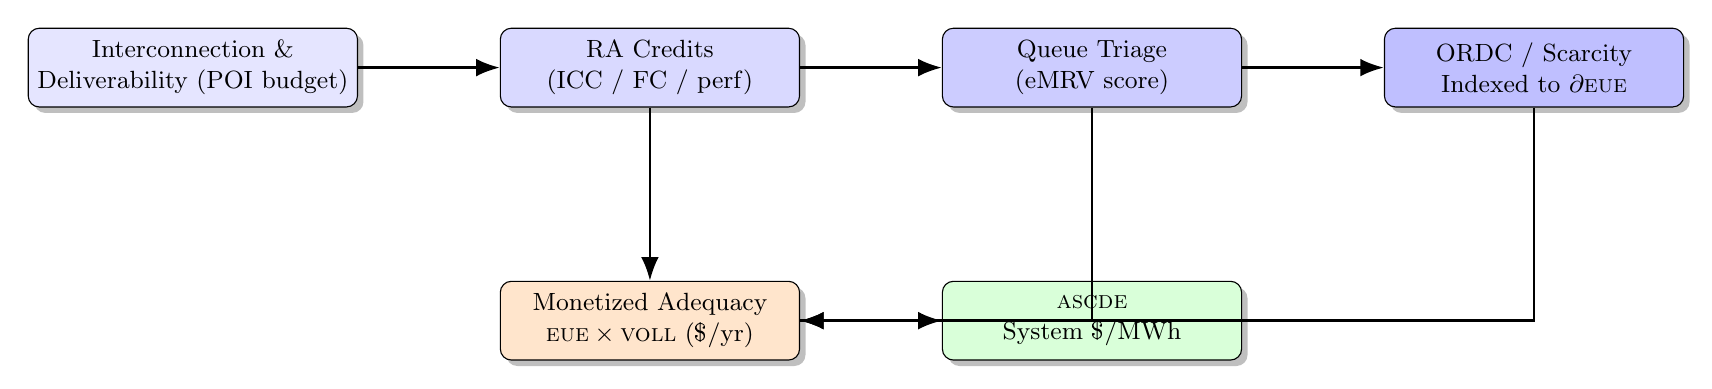
\begin{tikzpicture}[
  node distance=1.8cm,
  every node/.style={font=\small},
  blk/.style={draw, rounded corners, align=center, fill=gray!10, minimum width=38mm, minimum height=10mm, drop shadow},
  ar/.style={-{Latex[length=3mm]}, line width=0.9pt}
]
  % top chain
  \node[blk, fill=blue!10] (poi) {Interconnection \&\\Deliverability (POI budget)};
  \node[blk, right=of poi, fill=blue!15] (ra) {RA Credits\\(ICC / FC / perf)};
  \node[blk, right=of ra, fill=blue!20] (triage) {Queue Triage\\(eMRV score)};
  \node[blk, right=of triage, fill=blue!25] (ordc) {ORDC / Scarcity\\Indexed to $\partial \EUE$};

  \draw[ar] (poi) -- (ra);
  \draw[ar] (ra) -- (triage);
  \draw[ar] (triage) -- (ordc);

  % bottom target
  \node[blk, below=2.2cm of ra, fill=orange!20] (rv) {Monetized Adequacy\\$\EUE \times \VOLL$ (\$/yr)};
  \node[blk, right=of rv, fill=green!15] (ascde) {\ASCDE\\System \$/MWh};

  \draw[ar] (ordc.south) |- (rv.east);
  \draw[ar] (ra.south) -- (rv.north);
  \draw[ar] (triage.south) |- (rv.east);
  \draw[ar] (rv) -- (ascde);

\end{tikzpicture}%
}
\caption{Mechanism map: Interconnection \& deliverability, RA credits, queue triage, and EUE-indexed ORDC cohere around a single valuation basis (\EUE\,$\times$\,\VOLL) feeding \ASCDE.}
\end{figure}

%=============================
\section*{7Transmission and Interregional Policy}

\subsection{Locational Signals for AI Campuses}
\label{subsec:ai_loc}

\paragraph{eMRV maps for siting.} Publish seasonal \emph{eMRV heatmaps} identifying nodes/substations where an added MW most reduces \EUE{} (per \VOLL). Use these maps to guide large-load siting; campuses locating in high-eMRV zones receive streamlined interconnection and higher ICC multipliers; low-eMRV zones require cost sharing.

\paragraph{Upgrade cost sharing tied to avoided \EUE.} For network upgrades $u$ that increase $D_\ell$ and reduce \EUE{} by $\Delta \EUE_{u}$,
\[
\text{Reliability Benefit}_{u} \;=\; \Delta \EUE_{u} \times \VOLL,
\]
allocate upgrade costs to beneficiaries (e.g., hyperscale load + generators) pro-rata to realized reliability benefit. This aligns incentives without blunt socialization.

\paragraph{Grid-Enhancing Technologies (GETs).} Prioritize GETs (dynamic line ratings, topology optimization, power flow controllers) where $\Delta \EUE/\Delta \text{Cost}$ is largest. Compute \emph{temporary} $D_\ell$ uplift as a service; settle monthly against realized reductions in \EUE{}.

% --- eMRV Heatmap Mock TikZ ---
\begin{figure}[H]
\centering
\resizebox{0.9\textwidth}{!}{%
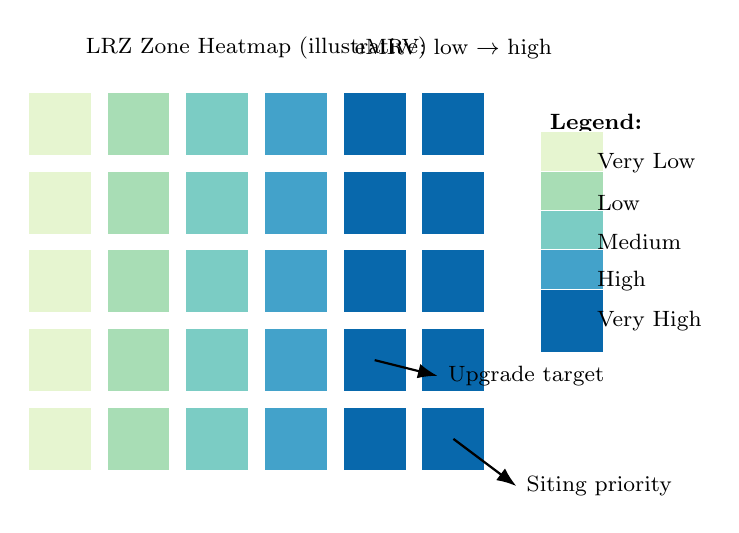
\begin{tikzpicture}[
  every node/.style={font=\small},
  cell/.style={rectangle, minimum width=8mm, minimum height=8mm, draw=white},
  lab/.style={font=\footnotesize}
]
  % color scale (low to high eMRV)
  \definecolor{cA}{RGB}{230,245,208}
  \definecolor{cB}{RGB}{168,221,181}
  \definecolor{cC}{RGB}{123,204,196}
  \definecolor{cD}{RGB}{67,162,202}
  \definecolor{cE}{RGB}{8,104,172}

  % simple 6x5 grid with increasing eMRV by column (illustrative)
  \foreach \y in {5,4,3,2,1}{
    \node[cell, fill=cA] at (1,\y) {};
    \node[cell, fill=cB] at (2,\y) {};
    \node[cell, fill=cC] at (3,\y) {};
    \node[cell, fill=cD] at (4,\y) {};
    \node[cell, fill=cE] at (5,\y) {};
    \node[cell, fill=cE] at (6,\y) {};
  }

  % labels
  \node[lab, above] at (3.5,5.7) {LRZ Zone Heatmap (illustrative)};
  \node[lab, above] at (6,5.7) {eMRV: low $\rightarrow$ high};

  % color legend
  \node[lab, right] at (7.1,5.0) {\textbf{Legend:}};
  \node[cell, fill=cA, right] at (7.1,4.5) {};
  \node[lab, right] at (7.7,4.5) {Very Low};
  \node[cell, fill=cB, right] at (7.1,4.0) {};
  \node[lab, right] at (7.7,4.0) {Low};
  \node[cell, fill=cC, right] at (7.1,3.5) {};
  \node[lab, right] at (7.7,3.5) {Medium};
  \node[cell, fill=cD, right] at (7.1,3.0) {};
  \node[lab, right] at (7.7,3.0) {High};
  \node[cell, fill=cE, right] at (7.1,2.5) {};
  \node[lab, right] at (7.7,2.5) {Very High};

  % annotation arrows
  \draw[-{Latex[length=2.5mm]}, thick] (6,1) -- ++(0.8,-0.6) node[lab, right] {Siting priority};
  \draw[-{Latex[length=2.5mm]}, thick] (5,2) -- ++(0.8,-0.2) node[lab, right] {Upgrade target};

\end{tikzpicture}%
}
\caption{Illustrative seasonal eMRV heatmap for siting signals (darker = higher eMRV).}
\end{figure}

% --- GETs schematic: ΔEUE benefit vs cost ---
\begin{figure}[H]
\centering
\resizebox{0.85\textwidth}{!}{%
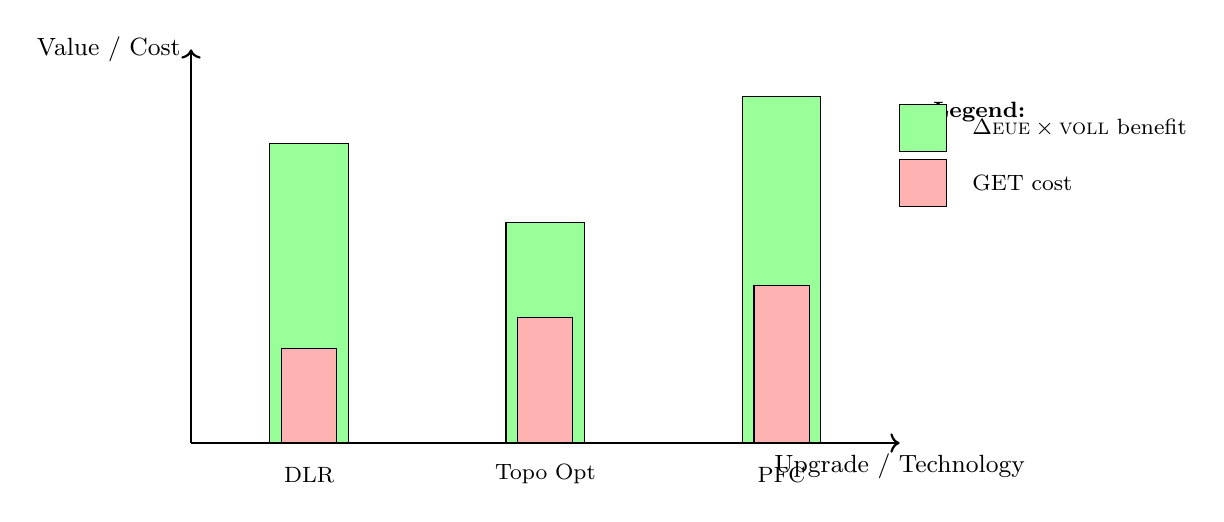
\begin{tikzpicture}[
  node distance=1.2cm,
  every node/.style={font=\small},
  axis/.style={->, thick},
  bar/.style={draw, fill=gray!30},
  lab/.style={font=\footnotesize}
]
  % axes
  \draw[axis] (0,0) -- (9,0) node[below] {Upgrade / Technology};
  \draw[axis] (0,0) -- (0,5) node[left] {Value / Cost};

  % x labels
  \node[lab] at (1.5,-0.4) {DLR};
  \node[lab] at (4.5,-0.4) {Topo Opt};
  \node[lab] at (7.5,-0.4) {PFC};

  % benefit (ΔEUE × VOLL)
  \draw[bar, fill=green!40] (1.0,0) rectangle (2.0,3.8);
  \draw[bar, fill=green!40] (4.0,0) rectangle (5.0,2.8);
  \draw[bar, fill=green!40] (7.0,0) rectangle (8.0,4.4);

  % cost bars (overlay thinner)
  \draw[bar, fill=red!30] (1.15,0) rectangle (1.85,1.2);
  \draw[bar, fill=red!30] (4.15,0) rectangle (4.85,1.6);
  \draw[bar, fill=red!30] (7.15,0) rectangle (7.85,2.0);

  % legend
  \node[lab, right] at (9.3,4.2) {\textbf{Legend:}};
  \draw[bar, fill=green!40] (9.0,3.7) rectangle (9.6,4.3);
  \node[lab, right] at (9.8,4.0) {$\Delta \EUE \times \VOLL$ benefit};
  \draw[bar, fill=red!30] (9.0,3.0) rectangle (9.6,3.6);
  \node[lab, right] at (9.8,3.3) {GET cost};

\end{tikzpicture}%
}
\caption{Grid-Enhancing Technologies (GETs): prioritize by highest $\Delta \EUE/\Delta\text{Cost}$ ratio.}
\end{figure}

\subsection{Interregional Transfer Capability as Reliability Asset}
\label{subsec:itc_asset}

\paragraph{Monetize transfer upgrades via \EUE.} For an interregional project $k$ that raises transfer capability by $\Delta T$ and reduces \EUE{} across regions by $\Delta \EUE_{k}$ (seasonal),
\[
\text{RB}_{k} \;=\; \Delta \EUE_{k} \times \VOLL,
\]
and include $\text{RB}_{k}$ as a first-class benefit alongside production cost savings in cost-benefit tests. Report native and standardized \VOLL{} values for transparency.

\paragraph{Seasonal firming agreements.} Allow bilateral seasonal hedges where Region A procures \emph{reliable import rights} from Region B (backed by transfer capability and resource accreditation) during A’s stress season. Price the contract at avoided \EUE{} value, settled ex post against realized scarcity.

\paragraph{Queue interaction.} Interregional projects with high $\text{RB}/\text{Cost}$ ratios should \emph{unlock} ARQ priority for co-dependent generation or large-load projects by jointly improving $D_\ell$ and MRV rankings across the seam.

\begin{tcolorbox}
\textbf{Policy hook:} Treat transfer capability as an adequacy resource: when priced via $\Delta \EUE\times\VOLL$, it competes fairly with new generation and load flexibility. This de-biases planning away from \emph{only} local buildout.
\end{tcolorbox}

%=============================
\section*{8 Regulatory Alignment}

This section maps the proposed \UEVF/\ASCDE framework and mechanism stack to current governance venues and responsibilities. The goal is to enable near-term adoption via guidance, reporting, and light-touch tariff/BPM updates.

\subsection{FERC, OMS, NARUC Touchpoints}

\paragraph{FERC.}
\begin{itemize}[leftmargin=1.25em]
  \item \textbf{Market rule guidance:} Encourage ISOs/RTOs to publish seasonal, locational \EUE{} bands and a standardized \VOLL{} range (e.g., 10–25 k\$/MWh) in RA and transmission filings; acknowledge \(\EUE\times\VOLL\) as a first-class benefit metric in cost–benefit analyses (CBA) for transmission and interconnection.
  \item \textbf{Scarcity pricing alignment:} Endorse ORDC designs indexed to probabilistic \EUE{} (Section~\ref{subsec:ordc}); ensure capacity constructs and scarcity adders are consistent with \UEVF{} valuation.
  \item \textbf{ARQ oversight:} Allow ISOs to fast-track interconnection (ARQ) when seasonal \LOLE/\EUE{} thresholds are breached; require public MRV/eMRV scorecards and sunset reviews.
\end{itemize}

\paragraph{OMS (Organization of MISO States).}
\begin{itemize}[leftmargin=1.25em]
  \item \textbf{Policy bridges:} Request seasonal \ASCDE{} module reporting in MISO RA filings; require \emph{Large-Load RA Class} guidelines (telemetry, forecastability, interruptibility slices, performance settlement).
  \item \textbf{Transmission scoring:} Ask MISO to add a \(\Delta\EUE\times\VOLL\) benefit term to MTEP for reliability and economic projects (native and standardized \VOLL).
  \item \textbf{Scorecards:} Direct MISO to publish quarterly eMRV maps and queue scorecards (top-decile projects, seasonal).
\end{itemize}

\paragraph{NARUC.}
\begin{itemize}[leftmargin=1.25em]
  \item \textbf{State IRPs:} Recommend state commissions require utilities to report \ASCDE{} with seasonal reliability modules and \(\EUE\times\VOLL\) bands; request that load flexibility (ICC, FC) be included as explicit resources in IRPs.
  \item \textbf{Cross-sector coordination:} Promote gas--electric and telecom--electric coordination via shared \EUE{} scenarios for common-mode failures; encourage joint seasonal firming agreements (Section~\ref{subsec:itc_asset}).
  \item \textbf{Consumer transparency:} Encourage publication of expected outage cost (\$/yr) by LRZ/zone alongside PRM/LOLE.
\end{itemize}

\begin{tcolorbox}
\textbf{Regulatory payoff:} A monetized adequacy ledger (\(\EUE\times\VOLL\)) and an “all-in” system metric (\ASCDE) unify planning, interconnection, and market design—reducing dispute cycles and improving cross-jurisdiction comparability.
\end{tcolorbox}

\subsection{Consistency with NERC Risk Recommendations}

\paragraph{Grid transformation.} \UEVF{} provides the energy/time/location adequacy lens called for by NERC, supplanting static PRM with severity-aware, monetized risk.

\paragraph{Resilience to extreme events.} Tail-risk weighting (CVaR) and seasonal \EUE{} bands operationalize NERC’s “resilience as recovery” posture.

\paragraph{Critical interdependencies.} Gas and communications outages are priced through increased \EUE{}, making interdependency risk visible in \(\EUE\times\VOLL\) and \ASCDE{}.

\paragraph{Energy policy volatility.} \UEVF{}’s uncertainty ledger quantifies policy and supply-chain volatility as risk premiums rather than qualitative caveats.

%=============================
\section*{9 Illustrative Case Studies}

We present three stylized case studies using the \UEVF/\ASCDE toolkit. They demonstrate: (i) queue prioritization by eMRV, (ii) seasonal adequacy impact from large-load flexibility, and (iii) the relative adequacy value of interregional transfer upgrades versus on-site flexibility.

\subsection{Queue Prioritization by eMRV}

\paragraph{Setup.} Consider three interconnection requests at nodes \(A,B,C\), each 100 MW, with seasonal deliverability factors \(D_\ell\) and marginal risk reductions measured as \(-\partial \EUE/\partial \text{Cap}\) from 1 MW finite differences.

\begin{center}
\begin{tabular}{lccc}
\toprule
 & Node A & Node B & Node C \\
\midrule
$D_\ell$ (deliverability) & 0.90 & 0.60 & 0.80 \\
$-\partial \EUE/\partial \text{Cap}$ (MWh/MW-yr) & 5.0 & 8.0 & 3.5 \\
\VOLL{} (\$/MWh) & 20{,}000 & 20{,}000 & 20{,}000 \\
\midrule
\(\text{MRV}=\) \(-\partial \EUE/\partial \text{Cap}\cdot \VOLL\) (\$/MW-yr) & 100{,}000 & 160{,}000 & 70{,}000 \\
\(\text{eMRV}=\text{MRV}\cdot D_\ell\) (\$/MW-yr) & \textbf{90{,}000} & 96{,}000 & 56{,}000 \\
\bottomrule
\end{tabular}
\end{center}

\paragraph{Result.} Node \(B\) has the highest MRV, but Node \(A\) nearly ties after deliverability (\(D_\ell\))—a different ranking than raw PRM/UCAP would produce. If \(\text{MC}_{\text{cap}}=80{,}000\) \$/MW-yr, then \(B\) and \(A\) both clear (\(\text{eMRV}> \text{MC}_{\text{cap}}\)), while \(C\) does not—providing a defensible ARQ ordering.

\subsection{Seasonal Adequacy with/without Flexible Large Load Credits}

\paragraph{Setup.} A 600 MW data-center cluster interconnects in a spring-stressed LRZ. Without flexibility, seasonal \(\EUE_{\text{spring}}=6{,}000\) MWh/yr. The campus offers:
\begin{itemize}[leftmargin=1.25em]
  \item \textbf{ICC}: 20\% interruptible (120 MW) in LOLE-weighted hours.
  \item \textbf{FC}: sub-hour telemetry; forecast error reduced from 5\% to 2\%.
\end{itemize}

\paragraph{Valuation.} Monte Carlo studies show:
\[
\Delta \EUE_{\text{ICC}} \approx -2{,}000\ \text{MWh/yr},\qquad
\Delta \EUE_{\text{FC}} \approx -300\ \text{MWh/yr}.
\]
At \VOLL{} = 20 k\$/MWh, avoided outage cost is \(\approx 46\) M\$/yr. If \(\text{eMRV}=90{,}000\ \$/\text{MW-yr}\) and \(\alpha_{\text{spring}}=0.5\), then
\[
\text{ICC}_{\text{spring}}=0.5\times 120=60\ \text{MW},\qquad
\Pi_{\text{ICC}}=60\times 90{,}000 = 5.4\ \text{M\$}.
\]
The remaining benefit is credited to FC/reserves. Seasonal \ASCDE{} for the zone falls as the reliability module shrinks—demonstrating that flexible load participation yields portfolio-level cost relief.

\subsection{Interregional Transfer Upgrade vs. Onsite Flexibility}

\paragraph{Setup.} Region \(R\) faces winter stress: \(\EUE_{\text{winter}}=8{,}000\) MWh/yr. Two interventions are evaluated:

\begin{enumerate}[leftmargin=1.25em]
  \item \textbf{Transfer upgrade} \(k\): add 500 MW from Region \(S\) to \(R\), yielding \(\Delta \EUE_{k} = -3{,}500\) MWh/yr; CAPEX amortized at 30 M\$/yr.
  \item \textbf{Onsite flexibility}: a portfolio of ICC + storage shifting yields \(\Delta \EUE_{\text{flex}} = -2{,}600\) MWh/yr; annualized cost 18 M\$/yr.
\end{enumerate}

\paragraph{Valuation.} With \VOLL{} = 20 k\$/MWh:
\[
\text{RB}_{k}=70\ \text{M\$}/\text{yr},\quad \text{RB}_{\text{flex}}=52\ \text{M\$}/\text{yr}.
\]
Both interventions are net-positive, but the upgrade delivers higher value. However, if \(\text{time-to-service}\) is 5 years for the line and 1 year for flexibility, the present value of avoided outage cost can favor flexibility as a \emph{bridge} until the line is in service. \ASCDE{} comparisons show that the combined pathway (flexibility now, transfer later) dominates either alone under most discount rates.

\begin{tcolorbox}
\textbf{Policy takeaway:} \UEVF{} lets ISOs and regulators treat transfers and flexibility on the same dollar scale. Seasonal \ASCDE{} and \(\EUE\times\VOLL\) reporting reveal the least-cost path to adequacy in time and space.
\end{tcolorbox}

%=============================
\section{Metrics, KPIs, and Compliance}

This section specifies how the proposed \UEVF--\ASCDE{} framework should be operationalized in practice. 
Metrics and key performance indicators (KPIs) must serve both as external accountability tools (public reporting, stakeholder oversight) and as internal compliance guardrails (ISO monitoring, settlement verification). 
The emphasis is on transparency, reproducibility, and comparability across regions.

\subsection{Public Scorecards}

\paragraph{Design.} 
Publish quarterly \emph{Resource Adequacy Scorecards} that report standardized indicators across ISOs, structured around:
\begin{enumerate}[label=(\alph*), leftmargin=*, itemsep=0.25em]
  \item \textbf{EUE outcomes:} realized unserved energy (MWh) and probability-weighted exceedance curves.
  \item \textbf{VOLL calibration:} documented values, sensitivity bands, and sectoral differentiation (residential, commercial, critical loads).
  \item \textbf{Reliability value (\(\EUE \times \VOLL\)):} annualized ledger of monetized outage risk (\$/yr).
  \item \textbf{ASCDE benchmarking:} reported \$/MWh ``all-in'' adequacy costs by portfolio/resource class, disaggregated into dispatch, storage, transmission, and market-value components.
  \item \textbf{Queue metrics:} interconnection backlog triage based on eMRV ranking; publication of nodal heatmaps showing highest marginal reliability value.
\end{enumerate}

\paragraph{Purpose.} 
The scorecards create a \emph{common language} for legislators, regulators, and market participants to evaluate adequacy investments. 
They also allow for cross-jurisdictional benchmarking (e.g., comparing MISO’s seasonal LOLE against CAISO’s flexible capacity margin) in a way that is interpretable to non-technical audiences.

\subsection{Bias/Uncertainty Ledger}

\paragraph{Motivation.}
Adequacy planning and RA markets are vulnerable to structural biases:
\begin{itemize}
  \item Forecast error in weather and load modeling.
  \item Resource accreditation asymmetries (e.g., over-crediting thermal units relative to variable renewables).
  \item Geographic bias in interconnection (favoring low-cost but low-deliverability sites).
  \item Market design biases (e.g., scarcity pricing caps that truncate reliability signals).
\end{itemize}

\paragraph{Ledger format.}
Require each ISO to maintain and publish an annual \emph{Bias/Uncertainty Ledger} documenting:
\begin{enumerate}[label=(\roman*)]
  \item Source of uncertainty or bias.
  \item Expected directional impact on \EUE{}, \VOLL{}, and ASCDE outcomes.
  \item Quantitative bounds (e.g., $\pm$ MWh EUE due to climate model variance).
  \item Planned corrective action or mitigation.
\end{enumerate}

\paragraph{Compliance.}
Regulators (FERC/OMS/NARUC) should mandate the Ledger as a compliance artifact akin to financial disclosures. 
Over time, this establishes an \emph{audit trail of epistemic risk} and creates institutional memory to prevent recurring blind spots.

%=============================
\section{Open Issues and Research Agenda}

While \UEVF{} and \ASCDE{} establish a harmonized valuation language, several research and policy frontiers remain unresolved. 
This section outlines priority topics for continued inquiry.

\paragraph{Cross-sector Shapley allocation.}
Current adequacy costs are borne largely by electricity consumers, but many adequacy drivers (data centers, hydrogen production, EV fast charging) span multiple sectors. 
A forward agenda is to extend Shapley-value methods to allocate \(\Delta\EUE \times \VOLL\) across electricity, fuels, and industrial users, ensuring fair cost causation and preventing cross-subsidization.

\paragraph{Cyber-resilience valuation.}
Traditional RA metrics ignore correlated cyber outages. 
Future research should embed probability-weighted cyber contingencies into \EUE{} distributions, pricing the resilience premium via \VOLL{} calibrated to digital-economy loads. 
This creates an explicit reliability market signal for investments in redundancy, encryption, and operational cyber defenses.

\paragraph{Gas-electric co-optimization.}
Thermal accreditation hinges on gas deliverability, yet gas and electricity operate under separate planning paradigms. 
A joint \UEVF{} ledger could:
\begin{itemize}
  \item Embed gas deliverability as a stochastic constraint in \EUE{} modeling.
  \item Monetize gas outages as induced electric EUE events.
  \item Align pipeline expansion economics with avoided electric outage cost.
\end{itemize}

\paragraph{AI-driven reliability forecasting.}
Emerging opportunities include use of ML/AI for probabilistic adequacy forecasts, integrating sub-hourly weather, distributed telemetry, and behavioral demand models. 
The research frontier lies in coupling AI forecasts with \UEVF{} settlement metrics, ensuring that gains in forecastability translate into measurable adequacy credits.

\paragraph{Interregional equity.}
Finally, questions remain on how interregional transfer capability should be priced across heterogeneous VOLL calibrations. 
A joint research program with NERC, RTOs, and national regulators is needed to test mechanisms that equitably price cross-border adequacy contributions.

\begin{tcolorbox}
\textbf{Research agenda summary:} A full-stack adequacy valuation requires advancing allocation theory (Shapley), systemic risk modeling (cyber, gas-electric), AI forecasting integration, and interregional equity. These topics define the next stage of \UEVF{} scholarship and practice.
\end{tcolorbox}

%=============================
\section{Conclusion}

This report has traced the evolution from probabilistic reliability metrics 
(\LOLE, \EUE) to a monetized adequacy framework grounded in \VOLL, producing 
a unified currency of risk that can be priced, settled, and allocated 
throughout the grid. By extending this logic into the Adjusted System-level 
Cost of Delivered Electricity (\ASCDE), we create a comprehensive “all-in” 
metric of delivered electricity that explicitly integrates dispatch, storage, 
transmission, and reliability layers. The result is a consistent accounting 
system for valuing both supply- and demand-side resources, including the 
rapidly growing class of engineered digital loads (AI campuses, hyperscale 
data centers, crypto clusters, and other blocky demand profiles).

\subsection{Key Contributions of this Framework}

\begin{itemize}
    \item \textbf{Monetized Reliability Value.} By defining Reliability Value 
    as $\EUE \times \VOLL$, the framework transforms abstract outage risk into 
    a transparent annualized ledger ($\$/yr$) directly comparable to capacity 
    procurement and transmission costs. 

    \item \textbf{System-Level Integration.} \ASCDE places reliability 
    alongside fuel, dispatch, storage, and transmission, producing a unified 
    $\$/MWh$ cost that can be reported to regulators, policymakers, and 
    market participants without fragmentation.

    \item \textbf{Marginal Reliability Value (MRV/eMRV).} By differentiating 
    $\EUE$ with respect to incremental capacity and weighting by \VOLL, 
    then adjusting for deliverability, the framework creates a ranking 
    function that can be applied to interconnection queues, RA portfolios, 
    and transmission upgrades. This provides a transparent and defensible 
    method for triage in overloaded queues.

    \item \textbf{Flexible Load Accreditation.} Engineered loads receive 
    performance-based credits for interruptibility, forecastability, and 
    controllability, tied explicitly to adequacy value rather than 
    static nameplate or generic demand-response labels.

    \item \textbf{Transmission as an Adequacy Resource.} By valuing 
    interregional transfer capability at $\Delta \EUE \times \VOLL$, 
    transfer projects, grid-enhancing technologies, and transmission upgrades 
    are treated equivalently to new generation or storage additions, de-biasing 
    planning away from “local only” solutions.
\end{itemize}

\subsection{Policy Alignment}

This framework does not exist in a vacuum. Its design complements and 
extends ongoing regulatory and operational initiatives:

\begin{itemize}
    \item \textbf{NERC Risk Taxonomy (2025).} Directly operationalizes 
    the RISC priorities on resource adequacy, extreme events, and 
    interdependency management by producing metrics that capture 
    both stochastic volatility and deterministic lumpiness of large 
    loads.

    \item \textbf{MISO BPMs.}  
    \begin{itemize}
        \item \emph{BPM-021 (Transmission Pricing):} Extends cost 
        allocation logic by integrating monetized reliability value 
        into upgrade cost-sharing and interregional transfer valuation.  
        \item \emph{BPM-026 (Demand Response):} Refines accreditation 
        by tying interruptible and forecastable load products to 
        MRV/eMRV values rather than static credits.  
    \end{itemize}

    \item \textbf{FERC and State Regulators.} Embeds a common valuation 
    language that can be applied across interconnection reforms, capacity 
    market rules, and transmission planning dockets, reducing the 
    fragmentation currently seen across ISO filings.

    \item \textbf{Technology Interface.} Recognizes that innovations such as 
    NVIDIA Spectrum-X, NCCL/MagnumIO, and AI-optimized data center fabrics 
    are no longer “IT-sector only” issues but directly impact load physics, 
    unit commitment, and adequacy metrics. Regulatory frameworks must evolve 
    accordingly.
\end{itemize}

\subsection{Immediate Next Steps for ISOs/RTOs}

Based on this analysis, several low-regret, high-value actions can be 
implemented in the near term:

\begin{enumerate}
    \item \textbf{Publish eMRV Heatmaps.} Release nodal/substation maps 
    showing where an added MW most reduces \EUE. This creates locational 
    transparency for developers, load siting, and policy.

    \item \textbf{Queue Scorecards.} Require interconnection applicants to 
    report project-specific MRV/eMRV values alongside cost estimates, 
    enabling triage based on reliability contribution per dollar.  

    \item \textbf{Flexible Load Accreditation Pilots.} Launch pilot 
    programs where large data centers or industrial loads can register 
    telemetry-driven interruptible and forecastable capacity, settled 
    against MRV-indexed credits.

    \item \textbf{Transmission Upgrade Valuation.} Incorporate 
    $\Delta \EUE \times \VOLL$ into cost-benefit analyses for regional 
    and interregional projects, ensuring that reliability benefits are 
    reported alongside production cost savings.

    \item \textbf{Public Reliability Scorecards.} Report system-wide 
    \EUE, \VOLL assumptions, and ASCDE benchmarks annually, creating 
    a transparent basis for public and regulatory trust.
\end{enumerate}

\subsection{Future Research Agenda}

Finally, while this paper sets out the scaffolding, further research 
is required to deepen and extend the approach:

\begin{itemize}
    \item \textbf{Cross-Sector Allocation.} Develop Shapley-style allocation 
    methods to apportion monetized adequacy benefits across generation, load, 
    storage, and transmission participants.

    \item \textbf{Extreme Event Tail-Risks.} Enhance MRV/eMRV by embedding 
    fat-tailed distributions of weather, fuel, and cyber shocks into \EUE 
    estimates, reflecting true system risk.

    \item \textbf{Gas–Electric Coordination.} Extend \UEVF{} to capture 
    the joint reliability of gas supply and electric adequacy, particularly 
    for winter-peaking regions.

    \item \textbf{Cyber-Resilience Valuation.} Explore integration of 
    probabilistic cyber risk models into adequacy valuation, monetizing 
    resilience investments in telemetry, encryption, and system hardening.

    \item \textbf{Global Benchmarking.} Compare U.S. implementations with 
    EU, UK, and Asian adequacy reforms to harmonize metrics and encourage 
    cross-jurisdictional learning.
\end{itemize}

\subsection{Closing Reflection}

Incentivizing what reduces monetized outage risk is the cleanest principle 
for aligning digital-era load growth with grid stability. \UEVF{} and 
\ASCDE{} do not prescribe technologies or market designs, but instead provide 
a \emph{valuation language} that makes reliability explicit, comparable, 
and tradable. With AI-driven demand growth accelerating, the cost of not 
acting will be far greater than the cost of reform. The opportunity before 
regulators, ISOs, and market participants is to move reliability economics 
from the realm of abstract probability into the concrete language of 
dollars, megawatts, and transparent ledgers.

%=============================
\section*{References}

\begin{enumerate}[label={[\arabic*]}]
    \item NERC (2025). \emph{Reliability Issues Steering Committee (RISC) Priorities Report}.
    \item MISO (2025). \emph{Business Practices Manual: Transmission Pricing (BPM-021-r18)}.
    \item MISO (2024). \emph{Business Practices Manual: Demand Response (BPM-026-r12)}.
    \item FERC Orders (2020--2025). \emph{Capacity market, transmission cost allocation, and interconnection reform dockets}.
    \item NVIDIA (2024--2025). \emph{Spectrum-X Architecture, NCCL/MagnumIO Technical Papers}.
    \item UEVF/ASCDE Working Papers (2024--2025). \emph{Probabilistic adequacy, monetized risk, and unified valuation methodology}.
\end{enumerate}

\appendix

%========================================================
\section{Mathematical Details}
\label{app:math}

\subsection{Preliminaries and Notation}
Let \(L_t\) denote load (MW) and \(C_t\) denote available firm capacity (MW) in interval \(t\) of length \(\Delta t\).
Define the \emph{curtailment process}
\[
U_t \;\coloneqq\; \max\{0,\, L_t - C_t\}\quad [\mathrm{MW}]\,,
\]
and the \emph{Expected Unserved Energy (EUE)}
\[
\EUE \;\coloneqq\; \mathbb{E}\!\left[\sum_{t=1}^{T} U_t\,\Delta t\right]\quad [\mathrm{MWh/yr}]\,,
\]
with expectation over stochastic drivers (forced outages, weather-driven VRE, transmission contingencies, etc.).
Let \(\VOLL\) denote Value of Lost Load \([\$/\mathrm{MWh}]\). The annual \emph{Reliability Value} (monetized outage cost) is
\[
\RV \;\coloneqq\; \EUE \times \VOLL \quad [\$/\mathrm{yr}]\,.
\]
For seasonal partitions \(\mathcal{S}\) (e.g., winter/summer/shoulders), write \(\EUE = \sum_{s\in\mathcal{S}} \EUE_s\) and analogously for \(\RV\).

We index capacity augmentation by a decision vector \(\bm{\kappa}\in\mathbb{R}^n_{\ge 0}\) (e.g., nodal MW additions, or portfolio components), and write \(\EUE(\bm{\kappa})\) when emphasizing dependence.

%--------------------------------------------------------
\subsection{Marginal Reliability Value (MRV) and eMRV}
\paragraph{MRV (system-wide).}
Define the \emph{marginal reliability value} of an incremental MW (perfectly deliverable) as
\[
\MRV(\bm{\kappa}) \;\coloneqq\; -\,\frac{\partial \EUE(\bm{\kappa})}{\partial K}\,\VOLL \quad [\$/\mathrm{MW\cdot yr}]\,,
\]
where \(K\) is a scalar capacity increment; for vector-valued decisions, use the gradient
\[
\nabla_{\bm{\kappa}} \RV(\bm{\kappa}) \;=\; \VOLL \,\nabla_{\bm{\kappa}}\EUE(\bm{\kappa}) \in \mathbb{R}^n\,,\qquad
\MRV_i \;=\; -\,\frac{\partial \EUE}{\partial \kappa_i}\,\VOLL\,.
\]
\emph{Units:} \(\partial \EUE/\partial \kappa_i\) has units \((\mathrm{MWh/yr})/(\mathrm{MW})=\mathrm{h/yr}\); multiplying by \(\VOLL\,[\$/\mathrm{MWh}]\) yields \(\$/(\mathrm{MW\cdot yr})\).

\paragraph{Deliverability and eMRV (locational).}
Let \(D_\ell\in[0,1]\) denote the deliverability factor for location \(\ell\) (Security Constrained deliverability in scarcity intervals).\footnote{If \(\ELCC\) is already derated for network constraints, avoid double counting by setting \(D_\ell=1\), cf. guardrails in App.~\ref{app:telemetry}.}
For a capacity increment \(\delta \kappa_\ell\) at node \(\ell\), the effective MW is \(\delta \kappa_\ell^{\mathrm{eff}}=D_\ell\,\delta \kappa_\ell\).
Define
\[
\mathrm{eMRV}_\ell \;\coloneqq\; -\,\frac{\partial \EUE}{\partial \kappa_\ell^{\mathrm{eff}}}\,\VOLL \;=\; -\,\frac{1}{D_\ell}\,\frac{\partial \EUE}{\partial \kappa_\ell}\,\VOLL \,,
\]
with the understanding that \(\partial \EUE/\partial \kappa_\ell\) is computed from a network-constrained, chronological adequacy model (sub-hourly or hourly).

\paragraph{With \(\ELCC\).}
Let a resource \(r\) with nameplate \(N_r\) have effective load carrying capability \(\ELCC_r\in[0,1]\) and deliverability \(D_r\in[0,1]\). A marginal nameplate increment \(\mathrm{d}N_r\) yields effective firm MW \(\mathrm{d}K_r = (\ELCC_r D_r)\,\mathrm{d}N_r\).
Then
\[
\frac{\partial \EUE}{\partial N_r} \;=\; \frac{\partial \EUE}{\partial K_r}\,(\ELCC_r D_r)
\quad\Rightarrow\quad
\MRV_{N_r} \;=\; -\,\frac{\partial \EUE}{\partial N_r}\,\VOLL
\;=\; -\,(\ELCC_r D_r)\,\frac{\partial \EUE}{\partial K_r}\,\VOLL\,.
\]
Thus project ranking in nameplate space is naturally proportional to \(\ELCC_r D_r\) times the MW‑based MRV.

%--------------------------------------------------------
\subsection{Properties of \(\EUE(\kappa)\)}

\begin{proposition}[Monotonicity and diminishing returns]
For any feasible expansion \(\bm{\kappa}\ge 0\), \(\EUE(\bm{\kappa})\) is nonincreasing in each component \(\kappa_i\) and piecewise convex with diminishing marginal benefits as adequacy saturates.
\end{proposition}

\begin{proof}[Sketch]
\emph{Nonincreasing:} Additional firm MW cannot increase unserved energy in any
scenario; hence the ensemble expectation is nonincreasing. \emph{Diminishing returns:}
as the probability mass of curtailment intervals shrinks, the measure of states in
which added MW binds declines, yielding smaller absolute gradient
$\bigl|\partial \EUE/\partial \kappa_i\bigr|$.
\end{proof}

%--------------------------------------------------------
\subsection{PRM optimality condition}
Let annual capacity cost (per MW‑yr) of technology \(j\) be \(\MC_j\). Consider a marginal change in planning reserve margin implemented via technology \(j\). The economically efficient PRM (first-order condition) satisfies
\[
\MC_j \;=\; \MRV_j \;=\; -\,\frac{\partial \EUE}{\partial \kappa_j}\,\VOLL\,.
\]
With multiple technologies, the condition holds for the infra‑marginal unit that sets the PRM increment.

%--------------------------------------------------------
\subsection{Seasonal ASCDE and reliability adders}
Let \(\mathcal{S}\) be a partition of the year into seasons \(s\), each with energy \(E_s\,[\mathrm{MWh}]\) and system cost \(C_s\,[\$]\) (including dispatch, fuel, storage, transmission, and reliability adder). Define seasonal \(\ASCDE\)
\[
\ASCDE_s \;\coloneqq\; \frac{C^{\text{non-rel}}_s}{E_s} \;+\; \underbrace{\frac{\EUE_s}{E_s}\,\VOLL}_{\text{seasonal reliability adder}}\quad [\$/\mathrm{MWh}]\,.
\]
The annual \(\ASCDE\) is an energy-weighted average:
\[
\ASCDE \;=\; \frac{\sum_{s\in\mathcal{S}} C^{\text{non-rel}}_s + \sum_{s\in\mathcal{S}} \EUE_s \VOLL}{\sum_{s\in\mathcal{S}} E_s}
\;=\; \sum_{s\in\mathcal{S}} w_s\,\ASCDE_s\,,\qquad w_s \;=\; \frac{E_s}{\sum_u E_u}\,.
\]
\paragraph{Per-season reliability adder.}
Define \(s_s \coloneqq \EUE_s/E_s\) as the share of seasonal energy at risk. The seasonal reliability adder is \(s_s \times \VOLL\) \([\$/\mathrm{MWh}]\).
If \(\VOLL\) varies by season (policy choice), substitute \(\VOLL_s\).

%--------------------------------------------------------
\subsection{Locational reliability price and settlement shadow prices}
In a constrained adequacy optimization, let \(\lambda_t\ge 0\) be the Lagrange multiplier on the nodal power balance/adequacy constraint capturing the marginal reliability (scarcity) value of 1 MW at time \(t\).
Then an approximation of the \emph{locational reliability price} is
\[
\pi^{\mathrm{rel}}_t \;\approx\; \VOLL \cdot \mathbb{P}(U_t>0) \quad [\$/\mathrm{MWh}]\,,
\]
or more generally \(\pi^{\mathrm{rel}}_t = \frac{\partial \RV}{\partial E_t}\) from the dual solution. Interval settlements for flexible load or storage providing adequacy support (curtailment/dispatch \(\delta E_t\)) then use
\[
\text{Credit}_t \;=\; \pi^{\mathrm{rel}}_t \,\delta E_t\,\Delta t\quad [\$].
\]
Aggregating across scarcity intervals yields consistency with annual \(\RV\) accounting.

%--------------------------------------------------------
\subsection{Computation pipeline and gradient estimation}
A practical pipeline for \(\MRV/\mathrm{eMRV}\) estimation:
\begin{enumerate}
  \item Run a baseline chronological, network-constrained adequacy simulation to obtain \(\EUE\) and per-interval curtailment sets.
  \item For each candidate location/technology \(i\), add a small firm MW increment \(\delta \kappa_i\) (respecting \(\ELCC_i D_i\)) and rerun (or use adjoint/sensitivity methods) to compute \(\Delta \EUE_i\).
  \item Estimate gradient: \(-\partial \EUE /\partial \kappa_i \approx (\EUE - \EUE^{(i)})/\delta \kappa_i\).
  \item Compute \(\MRV_i = -(\partial \EUE/\partial \kappa_i)\VOLL\); \(\mathrm{eMRV}_i = \MRV_i/D_i\) if deliverability not embedded.
\end{enumerate}

%========================================================
\section{Data Schemas and Telemetry}
\label{app:telemetry}

\subsection{Objectives and scope}
This appendix specifies the \emph{minimal data interface} for:
\begin{itemize}
  \item Ex‑ante forecasting used in commitment and adequacy (for large loads, storage, DR, and hybrid portfolios).
  \item Ex‑post telemetry used for settlement of flexibility products and performance-linked credits.
\end{itemize}
It is intentionally technology-neutral and consistent with ISO/RTO practice (granularity, latency, audit trail). The design supports:
(i) real-time validation, (ii) MRV/eMRV-indexed settlement, (iii) auditability (M\&V), and (iv) cyber integrity.

%--------------------------------------------------------
\subsection{Common timing, granularity, and synchronization}
\begin{itemize}
  \item \textbf{Interval length} \(\Delta t\): 5 minutes (minimum); 1‑minute optional sub-interval for validation; 15‑minute accepted where legacy constraints exist.
  \item \textbf{Forecast horizon}: day‑ahead (D‑1) hourly profile with sub-hourly refinement by H‑2; intra-day rolling forecast every 15 minutes with a 2‑hour lookahead.
  \item \textbf{Latency}: ex‑post telemetry delivered within 30 seconds of interval end; settlement-quality data within T\(+\)4 business days.
  \item \textbf{Clock synchronization}: PTP or NTP stratum‑1; maximum drift \(\le 100\) ms; signed timestamps in UTC with time zone offset.
\end{itemize}

%--------------------------------------------------------
\subsection{Entity model and identifiers}
\begin{tabular}{llp{8.7cm}}
\toprule
Field & Type & Description \\
\midrule
\texttt{resource\_id} & UUID & ISO‑assigned unique ID for resource/portfolio \\
\texttt{owner\_id} & UUID & Market participant identifier \\
\texttt{node} & string & Commercial pricing node or substation identifier \\
\texttt{resource\_type} & enum & \{\texttt{gen}, \texttt{stor}, \texttt{flex\_load}, \texttt{hybrid}\} \\
\texttt{nameplate\_mw} & float & Nameplate MW; for load, maximum curtailable MW \\
\texttt{elcc} & float & Effective Load Carrying Capability in \([0,1]\) if applicable \\
\texttt{deliverability} & float & \(D_\ell\in[0,1]\) seasonal or annual; if embedded in \ELCC, set to 1 \\
\texttt{portfolio\_operator} & UUID & Portfolio Operator of Record (if behind a POI portfolio) \\
\bottomrule
\end{tabular}

%--------------------------------------------------------
\subsection{Forecast API (ex‑ante)}
\paragraph{Endpoint.} \verb|POST /v1/forecast|
\paragraph{Payload schema (JSON).}
\begin{verbatim}
{
  "resource_id": "uuid",
  "version": "ISO-semver",
  "timestamp_utc": "2025-08-23T10:30:00Z",
  "forecast": [
    {
      "start_utc": "2025-08-24T00:00:00Z",
      "interval_min": 5,
      "mw": 12.34,
      "p10": 10.0,
      "p50": 12.3,
      "p90": 14.7,
      "status": "available|maintenance|derated",
      "event_flag": false
    },
    ...
  ],
  "signature": "base64-ecdsa"
}
\end{verbatim}
\emph{Notes.}
\begin{itemize}
  \item For \texttt{flex\_load}, \texttt{mw} is \emph{expected consumption}; curtailment capability reported in a parallel field \texttt{curtailable\_mw}.
  \item Probabilistic bounds (\texttt{p10/p50/p90}) required for H‑2 and closer; used for reserve sizing and bias detection.
  \item \texttt{status} communicates planned derates, forced outages, or maintenance windows.
\end{itemize}

%--------------------------------------------------------
\subsection{Telemetry API (ex‑post)}
\paragraph{Endpoint.} \verb|POST /v1/telemetry|
\paragraph{Payload schema (JSON).}
\begin{verbatim}
{
  "resource_id": "uuid",
  "timestamp_utc": "2025-08-24T00:05:00Z",
  "interval_min": 5,
  "meas": {
    "mw": 11.93,
    "voltage_kV": 230.1,
    "pf": 0.98
  },
  "quality": {
    "qflag": "good|estimated|bad",
    "missing_pct": 0.0,
    "latency_ms": 450
  },
  "signature": "base64-ecdsa"
}
\end{verbatim}

%--------------------------------------------------------
\subsection{Event/M\&V payloads}
For demand-side performance during declared scarcity events:
\begin{verbatim}
{
  "resource_id": "uuid",
  "event_id": "uuid",
  "intervals": [
    {
      "start_utc": "2025-08-24T21:00:00Z",
      "interval_min": 5,
      "baseline_mw": 25.1,
      "actual_mw": 18.7,
      "curtailment_mw": 6.4,
      "method": "CAISO-10of10|FSL|weather-adjusted",
      "confidence": 0.9
    }
  ],
  "signature": "base64-ecdsa"
}
\end{verbatim}
\emph{Baseline methods.} \texttt{FSL} (Firm Service Level), \texttt{10of10} with symmetric multiplicative adjustment, weather‑adjusted baselines for temperature‑sensitive loads.

%--------------------------------------------------------
\subsection{Validation and KPIs}
\begin{itemize}
  \item \textbf{Forecast accuracy:} Rolling MAPE and RMSE at daily and monthly horizons; threshold alarms at MAPE \(>15\%\) D‑1 or \(>10\%\) H‑2.
  \item \textbf{Telemetry quality:} Missing data \(<1\%\) per day; \texttt{qflag} \texttt{good} \(\ge 98\%\) intervals; latency \(<1\) s for operational, \(<\) 60 s for settlement streams.
  \item \textbf{Clock/sequence:} Reject non‑monotonic timestamps; require signed UTC and monotone sequence per \texttt{resource\_id}.
\end{itemize}

%--------------------------------------------------------
\subsection{Security and signing}
\begin{itemize}
  \item Mutual TLS; ECDSA signatures over \(\{\text{payload}, \text{timestamp}, \text{resource\_id}\}\).
  \item OAuth2 client credentials for API access; rotating keys with \(\le 90\) day rotation.
  \item Tamper‑evident logs: hash‑chained daily batch manifests (e.g., Merkle roots) retained \(\ge 7\) years.
\end{itemize}

%--------------------------------------------------------
\subsection{Settlement formulas (flexible load and storage)}
Let \(\pi^{\mathrm{rel}}_t\) be the per‑interval locational reliability price (scarcity/adequacy shadow price, cf. Sec.~\ref{app:math}), and \(\Delta E_t\,[\mathrm{MWh}]\) be delivered adequacy support (curtailment for load; discharge for storage).
\[
\text{Credit}_t \;=\; \pi^{\mathrm{rel}}_t \,\Delta E_t \,,\qquad
\text{Credit} \;=\; \sum_{t\in \mathcal{T}_{\mathrm{scar}}} \pi^{\mathrm{rel}}_t \,\Delta E_t\,.
\]
For portfolio‑level performance settlements, apply performance factor \(S_t\in[0,1]\) for telemetry quality and forecast compliance:
\[
\text{Paid}_t \;=\; S_t \cdot \text{Credit}_t,\qquad
S_t \;=\; S^{\mathrm{tele}}_t \cdot S^{\mathrm{fcst}}_t\,,
\]
where \(S^{\mathrm{tele}}_t\) penalizes \texttt{qflag} \(\neq\) \texttt{good} or excessive missingness; \(S^{\mathrm{fcst}}_t\) penalizes biased forecasts (\(|\text{err}|>\) threshold).

%--------------------------------------------------------
\subsection{Double‑counting guardrails}
\begin{enumerate}
  \item \textbf{Deliverability vs. transmission surcharge.} If \(\ELCC\) is computed with network constraints, set \(D=1\) and do not impose a separate upgrade surcharge in \(\ASCDE\).
  \item \textbf{Capacity vs. reliability credits.} For a given interval \(t\), a MWh cannot earn both energy/LMP and reliability/adequacy revenue for the \emph{same} service unless market rules explicitly co‑optimize and allocate shares.
  \item \textbf{Portfolio collisions.} Behind a single POI, the Portfolio Operator of Record must allocate per‑interval deliverability budgets to avoid exceeding \(D_{\ell,t}^{\text{budget}}\).
\end{enumerate}

%========================================================
\section{Illustrative Valuation Scenarios}
\label{app:valuation}

This appendix quantifies order‑of‑magnitude savings from applying the \UEVF/\ASCDE{} framework to hyperscale AI campuses that expose telemetry and controllability via AI‑optimized networking.
Numbers are \emph{illustrative}, based on stylized system assumptions chosen for transparency and to demonstrate the mechanics of the valuation.

\subsection{Methodology and Baseline Assumptions}
Let annual system energy be \(E_{\text{tot}}=\SI{300}{TWh}=\num{3.0e8}\,\text{MWh}\).
Let baseline expected unserved energy be \(\EUE_0=\SI{120000}{MWh/yr}\) (\(\approx 0.04\%\) of load), and take a harmonized \(\VOLL=\SI{10000}{\$/MWh}\) unless stated otherwise.
Baseline annualized outage cost (``reliability ledger'') is
\[
\RV_0 \;=\; \EUE_0\,\VOLL \,=\, \num{1.2e5}\times\num{1.0e4} \;=\; \SI{1.2e9}{\$/yr}.
\]
The \emph{reliability adder} in \$/MWh embedded in \ASCDE{} is
\[
\text{Adder}_0 \;=\; \frac{\EUE_0}{E_{\text{tot}}}\,\VOLL
\,=\, \frac{\num{1.2e5}}{\num{3.0e8}}\times \num{1.0e4}
\,\approx\, \SI{4.00}{\$/MWh}.
\]
Unless otherwise noted, the portfolio average \(\ASCDE_0\) (all‑in) is \SI{82}{\$/MWh}, of which \SI{4}{\$/MWh} is the reliability component and \SI{78}{\$/MWh} the non‑reliability component.

For a single \(\SI{500}{MW}\) campus that participates as a flexible load:
\begin{itemize}
  \item \textbf{ICC (interruptible capacity).} A fraction \(x\in[0,1]\) is curtailable in LOLE‑weighted intervals; seasonal/marginal \(\ELCC\) of the slice is \(\alpha\).
  \item \textbf{FC (forecastability credit).} Telemetry reduces reserve coverage and curtailment errors; we represent the net adequacy impact as a reduction \(\Delta\EUE_{\text{FC}}\).
\end{itemize}
We parameterize total adequacy effect as a percent reduction \(\rho\) in \(\EUE\):
\(\Delta \EUE = \rho\,\EUE_0\), yielding post‑intervention \(\EUE_1=(1-\rho)\EUE_0\).

\paragraph{Savings definitions.} 
\[
\text{RV Savings (\$)} \;=\; \Delta \RV 
= \Delta \EUE \times \VOLL
= \rho\,\EUE_0\,\VOLL
\]
\[
\text{RV Savings (\%)} \;=\; \frac{\Delta \RV}{\RV_0}\times 100 
= \rho \times 100.
\]
The reliability adder changes linearly with \(\EUE\):
\[
\text{Adder}_1 \,=\, \text{Adder}_0\,(1-\rho)
\quad\Rightarrow\quad
\Delta \text{Adder}\,(\$/\text{MWh}) = \rho\,\text{Adder}_0.
\]
Thus the new all‑in \(\ASCDE_1=\ASCDE_0 - \Delta \text{Adder}\).
Percent reduction in \ASCDE{} is \(\rho\times \text{Adder}_0/\ASCDE_0\).

\subsection{Scenario A: Interruptibility + Forecastability (ICC + FC)}
We consider three cases for total adequacy reduction \(\rho\): conservative (3\%), central (10\%), and stretch (25\%).
\begin{center}
\begin{threeparttable}
\caption*{Scenario A: Impact on monetized outage risk and \ASCDE{}}
\begin{tabular}{lrrrr}
\toprule
 & \textbf{Conservative} & \textbf{Central} & \textbf{Stretch} & \textbf{Units} \\
\midrule
\(\rho\) (EUE reduction) & \SI{3}{\percent} & \SI{10}{\percent} & \SI{25}{\percent} & \% of \(\EUE_0\) \\
\(\Delta \EUE\) & \num{3600} & \num{12000} & \num{30000} & MWh/yr \\
\(\Delta \RV=\Delta \EUE\times \VOLL\) & \SI{36}{M\$} & \SI{120}{M\$} & \SI{300}{M\$} & \$/yr \\
RV savings (\%) & \SI{3}{\percent} & \SI{10}{\percent} & \SI{25}{\percent} & of \(\RV_0\) \\
\(\Delta \text{Adder}\) & \SI{0.12}{\$/MWh} & \SI{0.40}{\$/MWh} & \SI{1.00}{\$/MWh} & \$/MWh \\
\(\ASCDE_1\) & \SI{81.88}{\$/MWh} & \SI{81.60}{\$/MWh} & \SI{81.00}{\$/MWh} & \$/MWh \\
\(\ASCDE\) savings (\%) & \SI{0.15}{\percent} & \SI{0.49}{\percent} & \SI{1.22}{\percent} & of \(\ASCDE_0\) \\
\bottomrule
\end{tabular}
\end{threeparttable}
\end{center}

\paragraph{Interpretation.}
Because the reliability adder is one component of \ASCDE{}, proportional reductions in \(\EUE\) translate one‑for‑one into proportional reductions of the adder, not the whole \ASCDE{}. Even so, a \(\SI{25}{\percent}\) adequacy improvement yields a \(\SI{1.22}{\percent}\) \ASCDE{} reduction and a large absolute reduction \((\SI{300}{M\$}/\text{yr})\) in the reliability ledger.

\subsection{Scenario B: Capacity Deferral Value via MRV/eMRV}
Suppose the nodal effective marginal reliability value is \(\mathrm{eMRV}=\SI{110000}{\$/MW\cdot yr}\).
If a campus provides interruptible capacity \(x=\SI{20}{\percent}\) on \(\SI{500}{MW}\) with seasonal \(\alpha=\SI{0.6}{}\), the accredited flexible MW is
\[
\text{ICC}=\alpha \times x \times \SI{500}{MW} = 0.6\times 0.2\times 500=\SI{60}{MW}.
\]
The annual credit at eMRV is \(\SI{60}{MW}\times\SI{110000}{\$/MW\cdot yr}=\SI{6.6}{M\$}/\text{yr}\).
If an equivalent peaker procurement costs \(\MC_{\text{cap}}=\SI{85000}{\$/MW\cdot yr}\), the avoided RA procurement is \(\SI{5.1}{M\$}/\text{yr}\).
\[
\text{Net benefit} = \SI{6.6}{M\$} - \SI{5.1}{M\$} = \SI{1.5}{M\$}/\text{yr},
\qquad
\text{Overcoverage} = \frac{6.6}{5.1}-1 \approx \SI{29}{\percent}.
\]
Thus, at this node, ICC credits can offset \(\approx\SI{129}{\percent}\) of equivalent peaker RA cost.

\subsection{Scenario C: Interregional Upgrade vs. Onsite Flexibility}
Let Region \(R\) be winter‑stressed: \(\EUE_{\text{winter}}=\SI{8000}{MWh/yr}\).
Consider two options:

\begin{enumerate}[label=(\roman*), leftmargin=1.25em]
  \item \textbf{Transfer upgrade} \(k\): \(\Delta T=\SI{500}{MW}\) raises import limits; \(\Delta \EUE_k=\SI{3500}{MWh/yr}\), annualized CAPEX \(\SI{30}{M\$}/\text{yr}\).
  \item \textbf{Onsite flexibility}: ICC + storage shift; \(\Delta \EUE_{\text{flex}}=\SI{2600}{MWh/yr}\), annualized cost \(\SI{18}{M\$}/\text{yr}\).
\end{enumerate}
At \(\VOLL=\SI{10000}{\$/MWh}\):
\[
\text{RB}_k=\SI{35}{M\$}/\text{yr},\quad \text{RB}_{\text{flex}}=\SI{26}{M\$}/\text{yr}.
\]
\[
\text{NPV margin}_k=(35-30)=\SI{5}{M\$}/\text{yr},\quad \text{NPV margin}_{\text{flex}}=(26-18)=\SI{8}{M\$}/\text{yr}.
\]
If \(\text{time-to-service}\) is 5 years for the line and 1 year for flexibility, the discounted avoided outage cost favors flexibility initially; the upgrade dominates long‑run if both are pursued. 
Percent reliability savings relative to winter ledger \((\EUE_{\text{winter}}\VOLL=\SI{80}{M\$}/\text{yr})\):
\[
\text{Savings}_k=\SI{43.8}{\percent},\qquad \text{Savings}_{\text{flex}}=\SI{32.5}{\percent}.
\]

\subsection{VOLL Sensitivity and Bands}
All reliability value results scale linearly with \(\VOLL\). For Scenario A (central, \(\rho=\SI{10}{\percent}\)):
\[
\Delta \RV(V)=\rho\,\EUE_0\,V,\qquad 
\frac{\mathrm{d}\,\Delta \RV}{\mathrm{d} V}=\rho\,\EUE_0=1.2\times 10^{4}\ \text{MWh/yr}.
\]
For \(\VOLL\in\{\SI{10000}{},\SI{17000}{},\SI{20000}{},\SI{25000}{}\}\,\$/\text{MWh}\), the central case saves \(\{\SI{120}{},\SI{204}{},\SI{240}{},\SI{300}{}\}\,\text{M\$}/\text{yr}\).
Publishing \(\VOLL\) bands ensures transparent robustness to policy choices about value of lost load.

\subsection{Summary Table of Savings (Selected Cases)}
\begin{center}
\begin{threeparttable}
\caption*{Illustrative savings in \$ and \% under \UEVF/\ASCDE{} incentives}
\begin{tabular}{lrrrr}
\toprule
 & \textbf{Conservative} & \textbf{Central} & \textbf{Stretch} & \textbf{Units} \\
\midrule
\multicolumn{5}{l}{\textit{Scenario A (ICC + FC)}}\\
RV savings & \SI{36}{M\$}/yr & \SI{120}{M\$}/yr & \SI{300}{M\$}/yr & \$/yr \\
RV savings (\%) & \SI{3}{\percent} & \SI{10}{\percent} & \SI{25}{\percent} & of \(\RV_0\) \\
\(\ASCDE\) savings & \SI{0.12}{\$/MWh} & \SI{0.40}{\$/MWh} & \SI{1.00}{\$/MWh} & \$/MWh \\
\(\ASCDE\) savings (\%) & \SI{0.15}{\percent} & \SI{0.49}{\percent} & \SI{1.22}{\percent} & of \(\ASCDE_0\) \\
\midrule
\multicolumn{5}{l}{\textit{Scenario B (ICC at eMRV)}}\\
ICC credit & \SI{6.6}{M\$}/yr & --- & --- & \$/yr \\
Avoided RA procurement & \SI{5.1}{M\$}/yr & --- & --- & \$/yr \\
Overcoverage & \SI{29}{\percent} & --- & --- & vs. peaker RA cost \\
\midrule
\multicolumn{5}{l}{\textit{Scenario C (Transfer vs Flex, winter)}}\\
RB (transfer) & \SI{35}{M\$}/yr & --- & --- & \$/yr \\
RB (flexibility) & \SI{26}{M\$}/yr & --- & --- & \$/yr \\
Winter RV savings & \SI{43.8}{\percent} & --- & --- & transfer vs \(\RV_{\text{winter}}\) \\
Winter RV savings & \SI{32.5}{\percent} & --- & --- & flexibility vs \(\RV_{\text{winter}}\) \\
\bottomrule
\end{tabular}
\end{threeparttable}
\end{center}

\begin{tcolorbox}
\textbf{Takeaway.} Even under conservative assumptions, telemetry‑backed interruptibility and forecastability can monetize \(\mathcal{O}(\$10^7)\) per campus annually in avoided outage costs and RA procurement, reduce all‑in \(\ASCDE{}\) by \(\sim 0.2\%{-}1.2\%\), and accelerate adequacy via eMRV‑based queue triage. With transfer upgrades priced at \(\Delta \EUE\times\VOLL\), on‑site flexibility serves as a high‑NPV bridge while long‑lead wires come online, with combined pathways delivering the lowest \(\ASCDE{}\) in most stress scenarios.
\end{tcolorbox}

\newpage

%========================================================
\section{Glossary}

\begin{description}
  \item[\(\ASCDE\) (Adjusted System‑level Cost of Delivered Electricity).] All‑in \(\$/\mathrm{MWh}\) cost including dispatch, fuel, storage, transmission, and monetized reliability (via \(\EUE\times\VOLL\)); seasonal variant \(\ASCDE_s\) uses seasonal energy and costs.

  \item[\(\EUE\) (Expected Unserved Energy).] Expected annual MWh of curtailed load from adequacy simulations; decomposed by season \(\EUE_s\) and/or by location.

  \item[\(\VOLL\) (Value of Lost Load).] Economic valuation of 1 MWh of unserved energy \([\$/\mathrm{MWh}]\); harmonized bands typically \(10{,}000\!-\!25{,}000\).

  \item[\(\RV\) (Reliability Value).] Annualized outage cost: \(\RV=\EUE\times\VOLL\) \([\$/\mathrm{yr}]\).

  \item[\(\LOLE\) (Loss of Load Expectation).] Expected number of days (or hours) per year with any shortage event (\(\le 0.1\) d/yr conventional criterion).

  \item[\(\MRV\) (Marginal Reliability Value).] \(\MRV = -(\partial \EUE/\partial K)\,\VOLL\) \([\$/\mathrm{MW\cdot yr}]\): avoided outage cost per incremental MW of firm capacity.

  \item[eMRV.] Deliverability‑adjusted MRV (locational or POI‑constrained): \(\mathrm{eMRV}=\MRV/D\) when deliverability is accounted ex‑post; if embedded in \ELCC, set \(D=1\).

  \item[\(\ELCC\) (Effective Load Carrying Capability).] Fraction \(\in[0,1]\) of nameplate treated as firm capacity for resource adequacy; may be seasonal/locational.

  \item[Deliverability factor (\(D\)).] Fraction \(\in[0,1]\) of accredited MW that can flow to the binding node under N‑1/N‑1‑1 during scarcity; time/season dependent.

  \item[PRM (Planning Reserve Margin).] \((\text{Capacity}-\text{Peak Load})/\text{Peak Load}\); chosen such that \(\MC=\MRV\) for marginal technology.

  \item[ORDC (Operating Reserve Demand Curve).] Scarcity pricing curve mapping reserve shortfall probability to price adder; may be indexed to probabilistic \(\EUE\).

  \item[Portfolio Operator of Record (POR).] Entity responsible for scheduling, telemetry, and deliverability allocation across co‑located resources behind a POI.

  \item[ICC (Interruptible Capacity Credit).] Performance‑linked capacity credit for large loads providing curtailable MW during scarcity; often settled vs. \(\pi^{\mathrm{rel}}_t\).

  \item[Forecastability Credit (FC).] Compensation for high‑fidelity probabilistic forecasts that reduce reserve needs; KPI‑linked (MAPE, bias).

  \item[Locational reliability price (\(\pi^{\mathrm{rel}}_t\)).] Per‑interval scarcity/adequacy shadow price used for settlements; conceptually \(\partial \RV/\partial E_t\).

  \item[GETs (Grid‑Enhancing Technologies).] DLR, topology optimization, power flow controllers; valued via \(\Delta \EUE \times \VOLL\).

  \item[FSL (Firm Service Level).] Baseline method for DR/LMR performance assessment: a pre‑agreed firm load level.

  \item[10of10 baseline.] Baseline method using average of ten most recent like‑days; often with symmetric multiplicative adjustment.

  \item[qflag.] Telemetry data quality flag: \texttt{good|estimated|bad}; used in settlement performance factors.

\end{description}

\end{document}
